\documentclass{article}
\usepackage[utf8]{inputenc}
\usepackage[linesnumbered, french,ruled,vlined]{algorithm2e}
\usepackage{listings}
\usepackage{xcolor}
\usepackage{graphicx}
\usepackage{siunitx}
\usepackage{amsfonts}
\usepackage{color}   %May be necessary if you want to color links
\usepackage{hyperref}
\usepackage[mathscr]{euscript}
\hypersetup{
    colorlinks=true, %set true if you want colored links
    linktoc=all,     %set to all if you want both sections and subsections linked
    linkcolor=blue,  %choose some color if you want links to ßstand out
}
%%%%    CHANGER mathsrc de euler en mathcal en gardant celui de LaTeX
%\let\mathcaltmp=\mathcal
%\let\mathscrtmp=\mathscr
%\usepackage{euler}
%\let\mathcal=\mathscr
%\let\mathscr=\mathscrtmp
%%%%
\usepackage[mathscr]{euscript}

\newcommand{\tsc}{\textsc}				%style capital
\newcommand{\mcl}{\mathcal}				%style semi-cursif
\newcommand{\scr}{\mathscr}				%style cursif
\newcommand{\M}{\mathfrak{M}}			%M matrices
\newcommand{\N}{\mathbb{N}}				%N naturels
\newcommand{\Z}{\mathbb{Z}}				%Z entiers relatifs
\newcommand{\Q}{\mathbb{Q}}				%Q fractionnels
\newcommand{\R}{\mathbb{R}}				%R réels
\newcommand{\Rn}{\R^n}			%R vécteurs
\newcommand{\Rnn}{\R^{n\times n}}			%R matrices carrées
\newcommand{\Rbar}{\overline{\R}}		%R barre, réels incluant infini
\newcommand{\C}{\mathbb{C}}				%C complexes
\newcommand{\K}{\mathbb{K}}				%K C ou R
\renewcommand{\P}{\mathscr{P}}			%P parties
\renewcommand{\L}{\mathscr{L}}			%L linéaire
\newcommand{\CC}{\mathscr{C}}			%C fonctions continues
\newcommand{\dd}{\text{d}}				%Dérivé (dt)
\newcommand{\Sc}{\scr{S}}				%S réels
\newcommand{\Cc}{\scr{C}}				%S réels
\newcommand{\D}{\scr{D}}			%P parties
\newcommand{\Y}{\scr{Y}}			%P parties
\newcommand{\X}{\scr{X}}			%P parties
\newcommand{\SPP}{\scr{S}_{++}^n}		%matrice sym def pos
\newcommand{\Eps}{\mathcal{E}}              %Eps
\newcommand{\norm}[1]{\left\lVert#1\right\rVert}
\newcommand{\cad}{\textbf{i.e :}}


\newcommand*\circled[1]{\tikz[baseline=(char.base)]{\node[shape=circle,draw,inner sep=1.5pt] (char) {#1};}}	%Entourer un caractère
\newcommand{\bam}{\begin{addmargin}[0.5cm]{0cm}}	%Ajouter l'indentation
\newcommand{\eam}{\end{addmargin}}		%Retirer l'indentation
\newcommand{\pmoins}{\scalebox{1}[1.0]{\( - \)}}	%Moins moins long
\newcommand{\ppmoins}{\scalebox{0.5}[1.0]{\( - \)}}	%Moins bien moins long
\newcommand{\fois}{\!\times\!}			%Multiplier, espaces raccourcis
\newcommand{\exist}{\exists\,}			%Il existe, espace droit augmenté
\newcommand{\findem}{\begin{flushright}\vspace{-0.35cm}$\square$\vspace{-0.2cm}\end{flushright}}	%Carré de fin de démonstration
\newcommand{\DE}{\textsc{d.e.}}			%Division euclidienne
\newcommand{\av}{\textsc{a.v.}{}}		%Au voisinage
\newcommand{\im}{\text{Im}}				%Image
\newcommand{\Ker}{\text{Ker}}			%Noyau
\newcommand{\sev}{\textsc{s-e.v.}}		%Sous-espace vectoriel
\newcommand{\Kev}{$\mathbb{K}$-\textsc{ev}}	%K-espace vectoriel
\newcommand{\rg}{\text{rg}}				%Rang
\newcommand{\Tr}{\text{Tr}}				%Trace
\newcommand{\Vect}{\text{Vect}}			%Vect
\newcommand{\diag}{\text{diag}}			%Diagonale (matrice)
\newcommand{\Card}{\text{Card}}			%Cardinal
\newcommand{\Id}{\text{Id}}				%Identité
\newcommand{\id}{\text{id}}				%Identité
\newcommand{\ul}{\underline}			%Souligner
\newcommand{\ol}{\overline}				%Sus-ligner
\newcommand{\tr}{\prescript{t}{}}		%Transposée
\newcommand{\com}{\footnotesize\ttfamily}	%Commentaire
\newcommand{\scol}{\setlength{\arraycolsep}{5pt}}	%Largeur colonnes large
\newcommand{\vect}{\overrightarrow}		%Sus-flecher
\newcommand{\ds}{\displaystyle}			%Forcer grand style
\newcommand{\scrotmp}{\mathchoice{{\scriptstyle\mathcal{O}}} {{\scriptstyle\mathcal{O}}} {{\scriptscriptstyle\mathcal{O}}} {\scalebox{.5}{$\scriptscriptstyle\mathscr{O}$}}}
\newcommand{\scro}{\scalebox{.8}[1.0]{$\scrotmp$}}%petit o manuscrit
\newcommand{\dlim}{\ds\lim}				%Limite avec indice en dessous
\newenvironment{psm}{\left(\begin{smallmatrix}}{\end{smallmatrix}\right)}	%Mini matrice

\makeatletter							%Flèche extensible
\newcommand{\xxrightarrow}[2][]{\ext@arrow 0359\xrightarrowfill@{#1}{#2}}
\newcommand{\xrightarrowfill@}{\arrowfill@\relbar\relbar{\mathrel{\smash{\rightarrow}\vphantom{\rightarrow}}}}
\makeatother

\makeatletter
\renewcommand{\o}[2][]{\scro_{#1}{\left(#2\right)}} %petit o de
\renewcommand{\O}[2][]{\mathcal{O}_{#1}{\left(#2\right)}} %grand o de
\newcommand{\simm}[1]{\,\underset{\raisebox{0.2ex}[0pt][0pt]{\scalebox{0.8}{$#1$}}}{\scalebox{1.1}[0.9]{$\sim$}}\,}			%équivalent à/simmilaire à
\newcommand{\restr}[2][]{{\left.\kern-\nulldelimiterspace #1\vphantom{\big|} \right|_{\scriptscriptstyle{#2}}}} 				%restreint à
\newcommand{\comp}[1]{{#1}^{\mathsf{c}}}		%Complémentaire
\makeatother

%%%%    REMISE DE mathcal (cf debut du fichier)
%\let\mathcal=\mathcaltmp

\definecolor{primaryColor}{rgb}{0.113, 0.364, 0.631}
\definecolor{primaryColor}{rgb}{0.6, 0.15, 0.18}
\definecolor{primaryColor}{rgb}{0.2, 0.45, 0.75}
\definecolor{secondaryColor}{rgb}{0.6, 0.6, 0,9}

\newcommand{\Exo}[2]{\vskip0.3cm\noindent \textcolor{primaryColor}{\textbf{Exercice #1 : #2 }}
\vskip0.2cm}

\usepackage{lipsum}
\usepackage{fancyhdr}
\usepackage{xcolor}

\usepackage{etoolbox}
\usepackage{amsmath,amsfonts,amssymb}
\usepackage[T1]{fontenc}

\definecolor{baseColor}{rgb}{0, 0.4, 1}
\definecolor{primaryColor}{HTML}{5c5554}
\definecolor{secondaryColor}{HTML}{101291}
\definecolor{successColor}{rgb}{0.02, 0.8, 0.25}
\definecolor{failColor}{rgb}{1, 0, 0}
\definecolor{mentionColor}{HTML}{dee3de}

\newcommand{\mention}[1]{\colorbox{mentionColor}{\textbf{#1}}}

\usepackage{tikz}
\usepackage{fontawesome}
\usepackage{geometry}
 \geometry{
 a4paper,
 total={170mm,257mm},
 left=20mm,
 right =20mm,
 top=20mm,
 }
\usepackage{fancyhdr}
\pagestyle{fancy}
\usepackage{titlesec}



\usepackage{blindtext}
\usepackage{fontawesome}

\usepackage[english]{babel}
\usepackage{tcolorbox}
\tcbuselibrary{minted,skins}

\newtcblisting{code}{
  listing engine=minted,
  colback=codebg,
  colframe=black!70,
  listing only,
  minted style=monokai,
  minted language=python,
  minted options={linenos=false,texcl=true},
  left=1mm,
}
\definecolor{codebg}{rgb}{0,0,0}
\usepackage{xcolor}

\begin{document}
\setcounter{secnumdepth}{4}
\titleformat{\paragraph}
{\normalfont\normalsize\bfseries}{\theparagraph}{1em}{}
\titlespacing*{\paragraph}
{0pt}{3.25ex plus 1ex minus .2ex}{1.5ex plus .2ex}

\begin{titlepage}
\lhead{\textcolor{primaryColor}{Projet ML 2020/2021}}

\newcommand{\HRule}{\rule{\linewidth}{0.5mm}} 

\center
 
%----------------------------------------------------------------------------------------
%	HEADING SECTIONS
%----------------------------------------------------------------------------------------



\includegraphics[width=13cm,height=3cm]{src/img/upd.png}\\
\textsc{\large M1-I2D}\\[0.5cm] 
\textsc{\Large Projet Data Science \& Machine Learning}\\[1.5cm] 


%----------------------------------------------------------------------------------------
%	TITLE SECTION
%----------------------------------------------------------------------------------------

\HRule \\[0.4cm]
{ \huge \bfseries Amazon Reviews Analysis}\\[0.4cm] 
\HRule \\[1.5cm]
 
%----------------------------------------------------------------------------------------
%	AUTHOR SECTION
%----------------------------------------------------------------------------------------

\begin{minipage}{0.4\textwidth}
\begin{flushleft} \large
\emph{\textbf{By :}}\\
Benamara \textsc{Abdelkader} 
\end{flushleft}
\end{minipage}
~
\begin{minipage}{0.4\textwidth}
\begin{flushright} \large
Djelid \textsc{Aymen}
\end{flushright}
\end{minipage}\\[1cm]

\begin{minipage}{0.4\textwidth}
\begin{flushleft} \large
\emph{\textbf{Supervisors :}}\\
Yger \textsc{Florian} 
\end{flushleft}
\end{minipage}
~
\begin{minipage}{0.4\textwidth}
\begin{flushright} \large
Borias \textsc{Nicolas}
\end{flushright}
\end{minipage}\\[2cm]


%----------------------------------------------------------------------------------------
%	DATE SECTION
%----------------------------------------------------------------------------------------


{\large May 8, 2021}\\[2cm]
Check our code on {\href{https://github.com/ChihabEddine98/AdvancedAlgos}
{ \textcolor{secondaryColor}{(Github)} \textcolor{black}{\faGithub} }}  




\vfill 

\end{titlepage}

%----------------------------------------------------------------------------------------
%	Table of contents
%----------------------------------------------------------------------------------------
\renewcommand{\contentsname}{Contents}
\hspace{1.5cm}
\hrule
{
  \hypersetup{linkcolor=secondaryColor}
  \tableofcontents
}
\hspace{1.5cm}
\hrule


\newpage
%----------------------------------------------------------------------------------------
%	Introduction
%----------------------------------------------------------------------------------------

\section*{Introduction :}

Sentiment analysis refers to analyzing an opinion or feelings about something using data like text or images, regarding almost anything. Sentiment analysis helps companies in their decision-making process. For instance, if public sentiment towards a product is not so good, a company may try to modify the product or stop the production altogether in order to avoid any losses.

There are many sources of public sentiment e.g. public interviews, opinion polls,.... etc, In this article, we are interested in the reviews of the products in  Amazone Website which is a big platform that contain several's of products from different brands like :Microsoft,Belei,Amazonfresh,revly....etc.we know that there are so many new products are emerging every day in this French website. Therefore, customers need to rely largely on product reviews to make up their minds for better decision making on purchase.However, searching and comparing text reviews can be frustrating for users. Hence we need better numerical ratings system based on the reviews which will make customers purchase decision with ease.

%----------------------------------------------------------------------------------------
%	Data Gathering
%----------------------------------------------------------------------------------------



\section{Data Gathering :}
\subsection{Dataset Choice : }
We decided to scrape the \textcolor{blue}{\faAmazon} \textbf{Amazon's} website and get user reviews data. So a simple way to define web scraping , is a process of automating the extraction of data in an efficient and fast way. With the help of web scraping, you can extract data from any website, no matter how large is the data, on your computer. In simple terms, web scraping saves you the trouble of manually downloading or copying any data and automates the whole process.\\
The following figure show us what our code will scrape from a given review.\\
\begin{figure}[H]
    \centering
    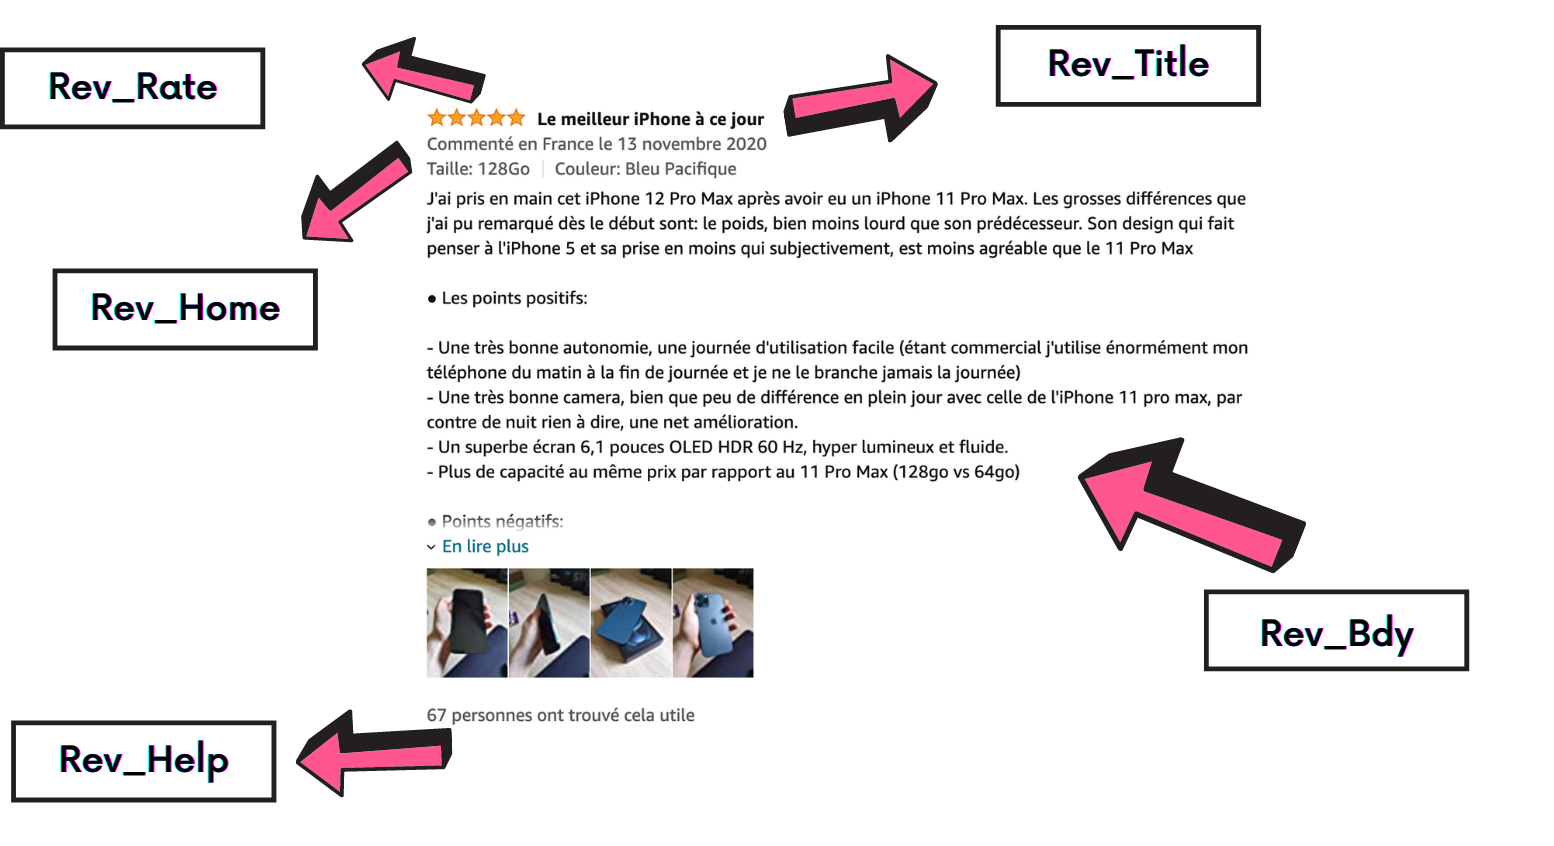
\includegraphics[scale=0.3]{src/img/amazon_review.png}
    \caption{Scraped Data from an Amazon- Review}
    \label{fig:my_label}
\end{figure}
In our project we used the library \mention{beautiful-soup} to scrape these reviews from the \textbf{Amazon's} website , and to do so we created this \mention{reviews\_scrapper} function which will help us to collect get needed and specific information that we're interested in : \\
\begin{code}
# Scrapping Reviews Data
def reviews_scrapper(driver, prod, rev_url, ds):
    driver.get(rev_url)
    rev_soup = BeautifulSoup(driver.page_source, 'html.parser')
    reviews_div = rev_soup.find_all('div', {'class': reviews_div_cls})

    for review in reviews_div:
        review_title = review.find('a', {'data-hook': 'review-title'}).text
        review_rate = review.find('i', {'data-hook': 'review-star-rating'}).text
        review_body = review.find('span', {'data-hook': 'review-body'}).text
        review_help = review.find('span', {'data-hook': 'helpful-vote-statement'}).text
        review_home = review.find('span', {'data-hook': 'review-date'}).text
        rev_result = tuple(map(lambda x:
                               unicodedata.normalize("NFKD", x.strip()),
                               [review_title, review_rate, review_body,
                                review_help, review_home]))
        ds.append(rev_result + (prod,))

    return ds
\end{code}
\noindent\\
So as shown in the previous function for all reviews in the amazon page we are going to create a tuple with wanted information and for missing data ( for example a missing help or missing title we replaced it by an \textbf{na-value} which will be handled in coming sections).\\
After the process of scraping we get this dataset which we stored in a \mention{csv}-file here we have its first 10 rows :
\begin{figure}[H]
    \centering
    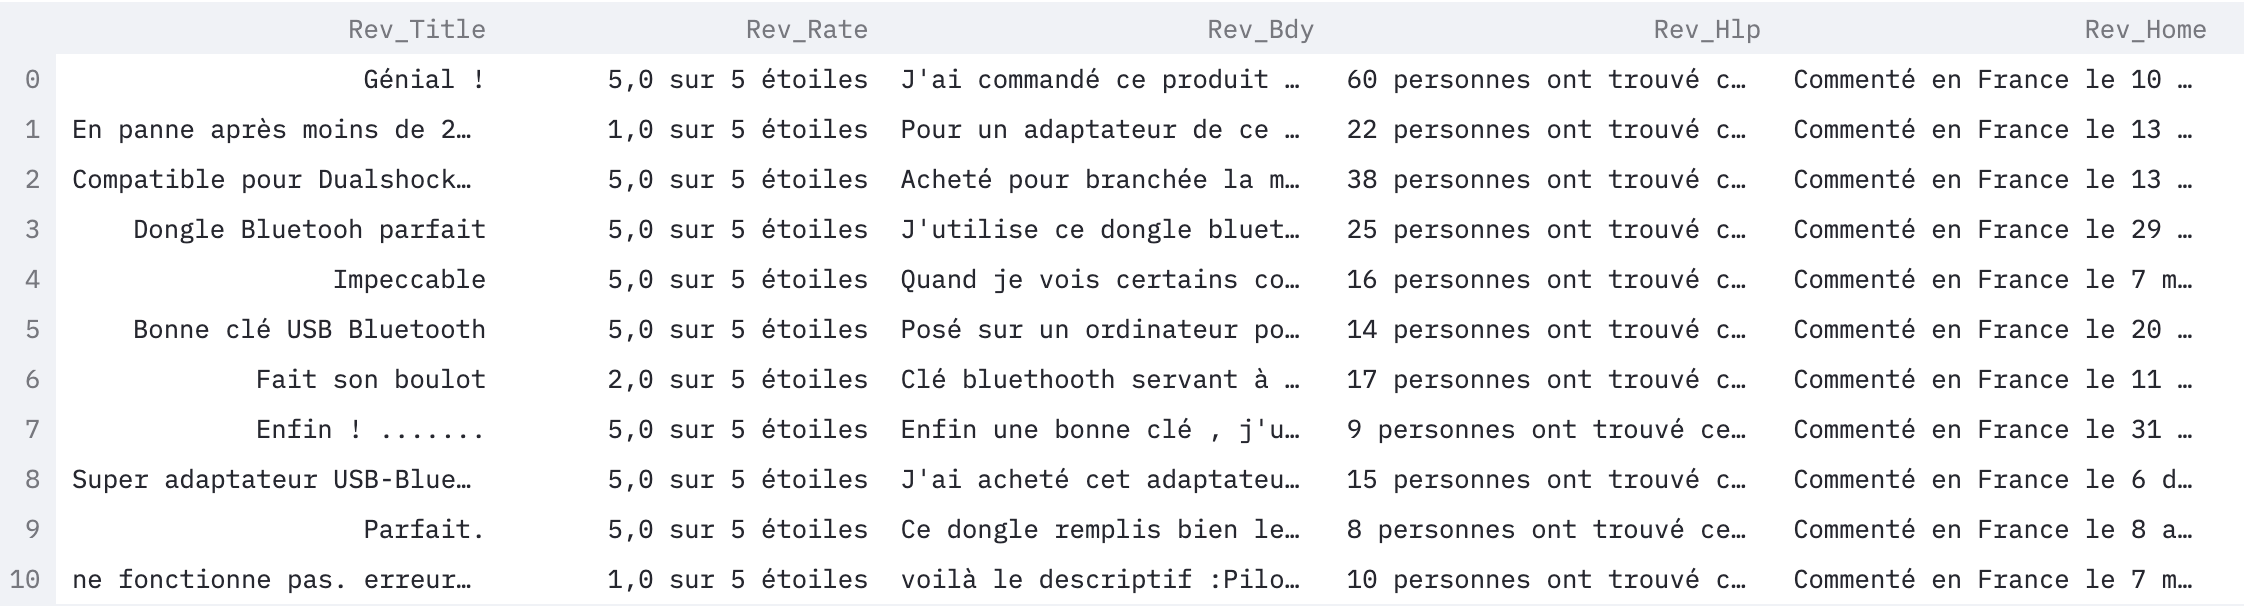
\includegraphics[scale=0.46]{src/img/dataset.png}
    \caption{Amazon Reviews Dataset}
    \label{fig:my_label}
\end{figure}

\section{Problem Defintion :}
\subsection{Tasks to solve :}
Given \textbf{Amazon's} reviews about several products of different categories and brands for example ( In category 'Tech' we can have many different products (Laptops, Smartphones , headphones ,$\dots$ ) The following show how we structured this on a dictionary :  \\
\begin{code}
'''
    Each Page of reviews contains 10 comments ( So if we took for
     example 100 rev_pages we are talking about 1000 comment )
'''

{
    # Category :
    'informatique':
    # List of products in this category
    [
        {
            'prod_id': 1,
            'prod_url': 'link-to-product-1-page',
            'rev_url': 'link-to-reviews-page',
            'rev_pages': 100,
        },
        {
            'prod_id': 2,
            'prod_url': 'link-to-product-2-page',
            'rev_url': 'link-to-review-page',
            'rev_pages': 'how-many-pages-of-reviews',
        },
    ]
}
\end{code}
\noindent The task is to predict whether a review  contains positive, negative, or neutral sentiment about the product. This is a typical \textbf{Supervised Learning} task where given a text string, we have to categorize the text string into predefined categories (3 in our case) We are talking about multi-class classification.\\
\textbf{Note : } We will be giving this encoding to our 3 classes, by \textbf{1} we refer to positive reviews , \textbf{-1} negative one's and by \textbf{0} neutral reviews.

\section{ Methodology Description : }
The methodolgy for this NLP project ( Sentiment Analysis ) is as shown in the following scheme :
\begin{figure}[H]
    \centering
    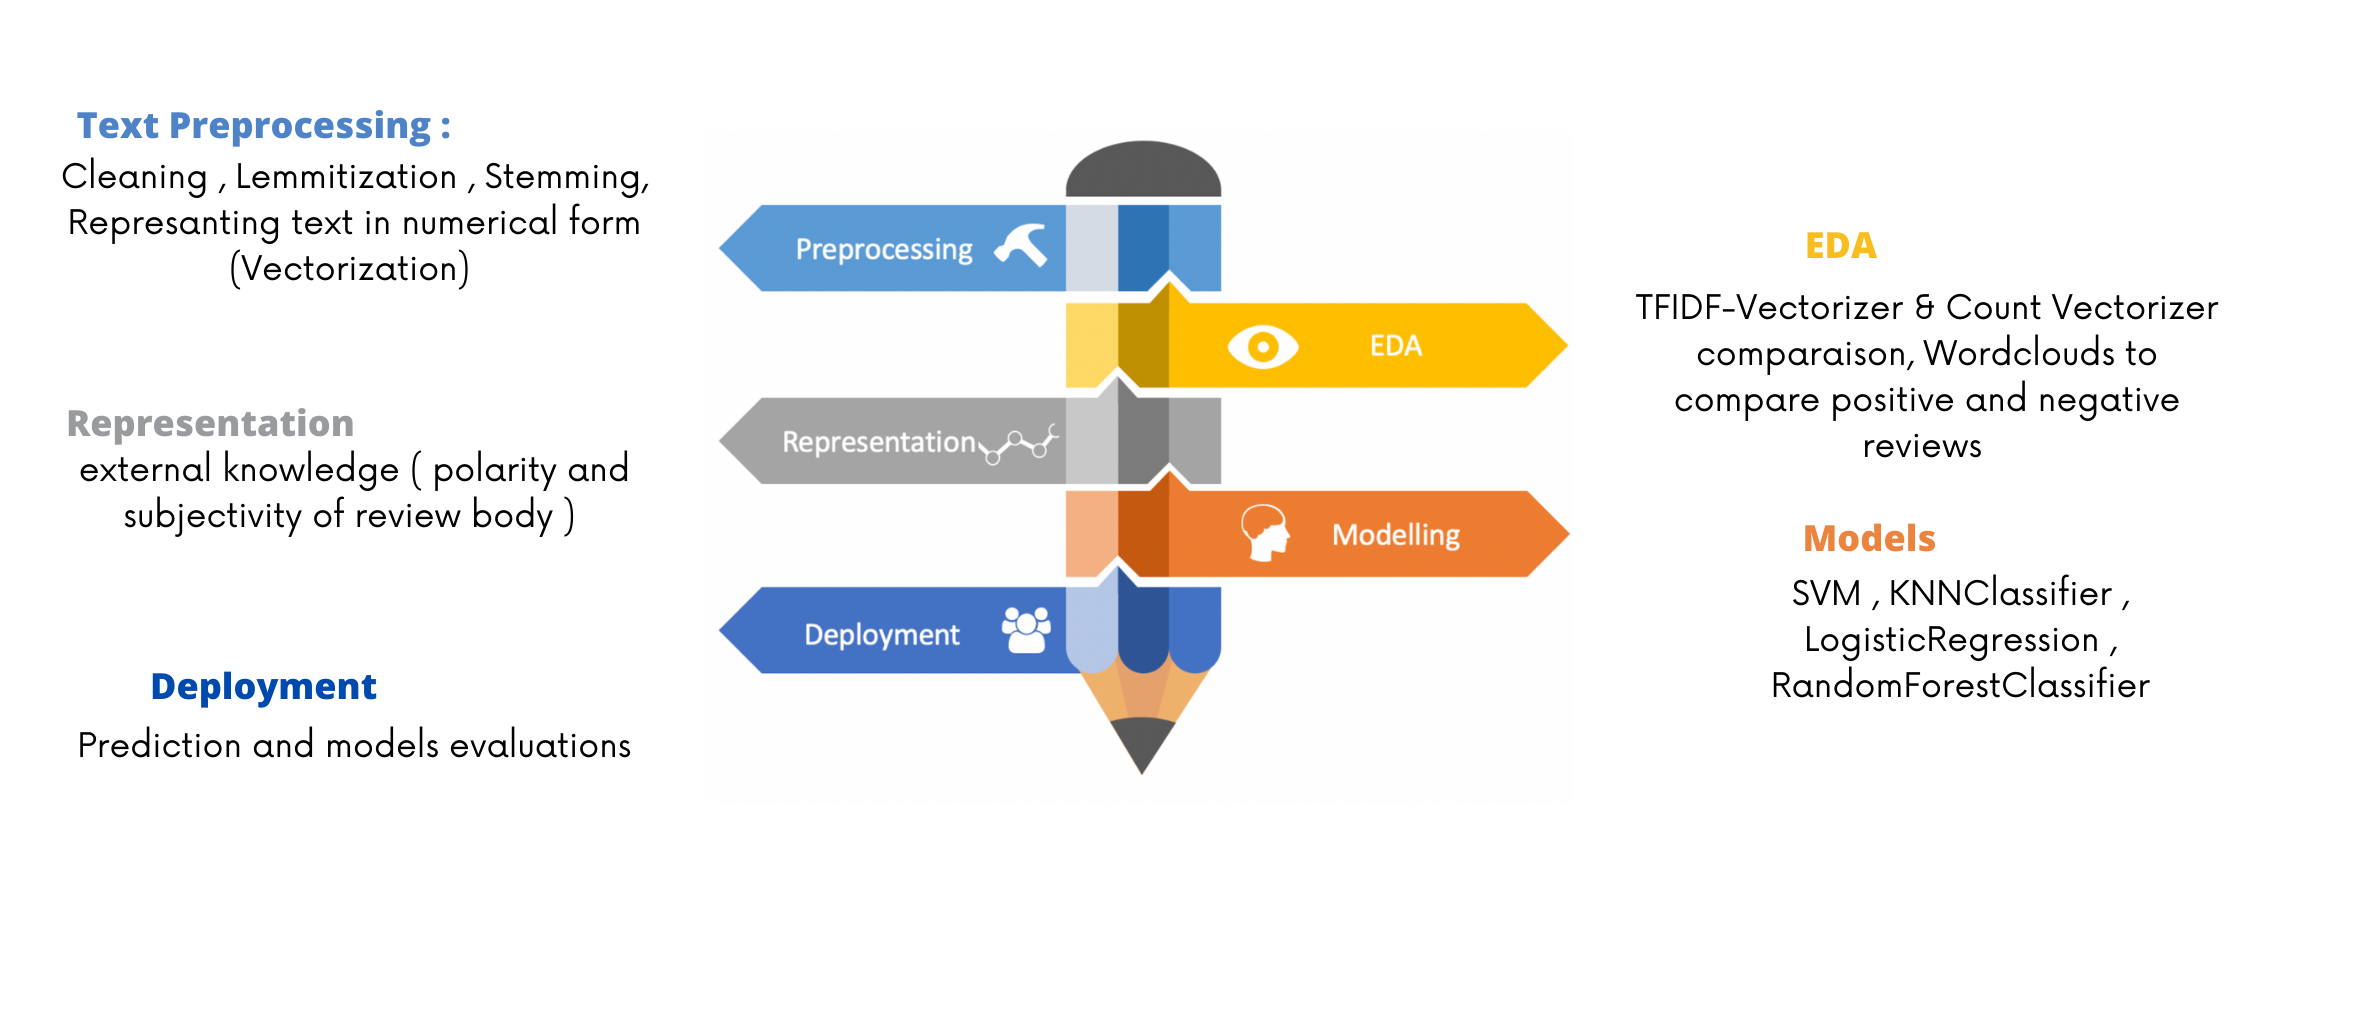
\includegraphics[scale=0.3]{src/img/methodology.png}
    \label{fig:my_label}
\end{figure}
\section{Dataset Analysis : }
\subsection{ Data Pre-processing : }
Since, text is the most unstructured form of all the available data, various types of noise are present in it and the data is not readily analyzable without any pre-processing. The entire process of cleaning and standardization of text, making it noise-free and ready for analysis is known as text preprocessing.\\
In this section, the following text preprocessing were applied on each row from the dataset.
\begin{enumerate}
    \item \textbf{Rev\_Rate :} here is an example of the original scraped data for this column : \textbf{(5,0 sur 5 étoiles)} and after cleaning we get just \textbf{float(5.0)} for this same row. This transformation is due to the following code
\begin{code}
    # Cleaning Rate review
    Rev_Rate = Rev_Rate.str.split(' ').apply(lambda x: float(x[0].replace(',','.')))
\end{code}
    \item \textbf{Rev\_Help :} here is an example of the original scraped data for this column : \textbf{(60 personnes ont trouvé ça utile)} and after cleaning we get just \textbf{int(60)} for this same row. This transformation is due to the following code
\begin{code}
    # Cleaning Hlp Review
    Rev_Hlp = Rev_Hlp.apply(lambda x: int(re.sub("[^0-9]","",x)))
\end{code}
    \item \textbf{Rev\_Home :} here is an example of the original scraped data for this column : \textbf{(Commenté en France le 20 Novembre 2020)} and after cleaning we get just \textbf{'France'} for this same row. This transformation is due to the following code
\begin{code}
    # Cleaning Home Review
    Rev_Home = Rev_Home.str.split(' ').apply(lambda x: x[2])
\end{code}
    \item \textbf{Rev\_Bdy :} This is the most important part of our cleaning process because all sentiment analysis will be based on the review body we can summarize the cleaning steps for the review body with the following function :
\begin{code}
# Clean Review Body
def clean_review_body(rev):
  # Make text to lowerCase
  clean_rev = rev.lower()
  # Remove ponctuation like .,!? etc
  clean_rev = clean_rev.translate(str.maketrans('','',string.punctuation))
  # Remove words that contain numbers
  clean_rev = re.sub(r'\w*\d\w*','',clean_rev)
  return clean_rev
\end{code}
\noindent
After this previous steps of cleaning we need to drop all rows that are not commented in France ( French Analysis only ).\\
Applying this steps to our original dataset produce the following dataset :
\begin{figure}[H]
    \centering
    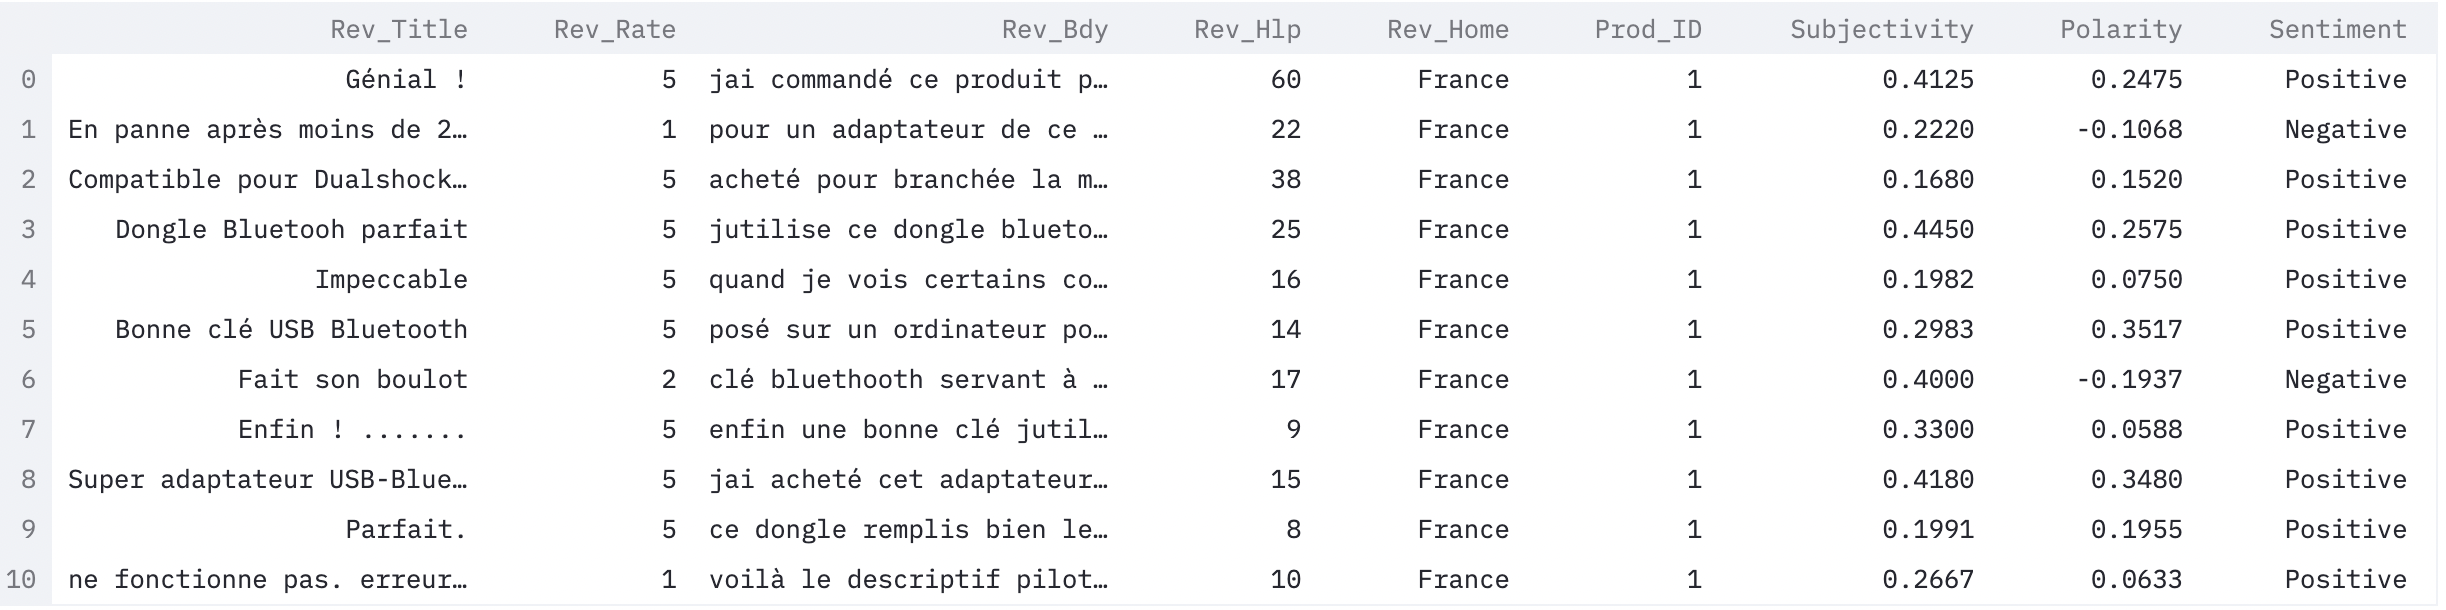
\includegraphics[scale=0.42]{src/img/clean_dataset.png}
    \caption{Amazon Reviews pre-processed Dataset}
    \label{fig:my_label}
\end{figure}

\subsubsection{Stemming \& Lemmitization :}
In this section we have to treat out \textbf{Stemming} subject which basically just removes or stems the last few characters of a word, often leading to incorrect meanings and spelling (for example \textbf{sel, saler, salière}) we would like to get have just one word in our data (\textbf{sel} for example) and this task is done in stemming section, in the other hand \textbf{Lemmatization} considers the context and converts the word to its meaningful base form, which is called Lemma. Sometimes, the same word can have multiple different Lemmas. We should identify the Part of Speech (POS) tag for the word in that specific context.\\
Lemmatization links words with similar meaning to one word. Wordnet and treebank have different tagging systems, so we want to first define a mapping between wordnet tags and POS tags. Then, we lemmatize words using NLTK.\\
This two tasks are so important to vectorize our data and also to genrate wordcloud in EDA sections.

\subsubsection{ Representing Text in Numerical Format (Vectorization) : }
Statistical algorithms use mathematics to train machine learning models. However, mathematics only work with numbers. To make statistical algorithms work with text, we first have to convert text to numbers. To do so, two main approaches exist \textbf{i.e.}  \textbf{TF-IDF} and \textbf{CountVectorizer} . In this section, we will discuss the \textbf{TF-IDF} scheme.\\
\mention{TF} computes the classic number of times the word appears in the text, and \mention{IDF} computes the relative importance of this word which depends on how many texts the word can be found. \mention{TF-DF} is the inverse document frequency. It adjusts for the fact that some words appear more frequently in general, like "Je", "Moi", etc. We discard words that appeared in > 90\% of the reviews and words appeared in < 10\% reviews since high appearing words are too common to be meaningful in topics and low appearing words won’t have a strong enough signal and might even introduce noise to our model.\\
Luckily for us, Python's \mention{Scikit-Learn} library contains the \textbf{TfidfVectorizer} class that can be used to convert text features into \textbf{TF-IDF} feature vectors. The following script performs this :
\begin{code}
stopwords = stopwords.words('french')

def data_to_matrix(data):
  # Building the Victorizer
  stemmer = FrenchStemmer()
  analyzer = TfidfVectorizer().build_analyzer()
  vec = TfidfVectorizer(stop_words = stopwords,
                        analyzer = lambda doc:(stemmer.stem(w) for w in analyzer(doc)),
                        ngram_range = (1,3))
  # Build the new matrix dataset
  mx_rev = vec.fit_transform(data.Rev_Bdy)
  df_rev = pd.DataFrame(mx_rev.toarray(),columns = vec.get_feature_names())
  df_rev.index = data.index
  df_rev.insert(0, 'Title', data.Rev_Title)
  return df_rev
\end{code}

\end{enumerate}


\subsection{ Statistical Analysis (EDA) :  }
\subsubsection{ Which Ratings got Highest Number of Reviews ? }
Customers have written reviews and ratings were given from 1 to 5 for Products they bought from Amazon. The distribution and percentage of ratings vs number of reviews is shown below. Number of reviews for rating 5 were high compared to other ratings. Overall, customers were happy about the products they purchased. About 79\% customers gave 5 rating for the products they purchased. Only about 8\% customers gave ratings less than 3 stars on their ratings.

\begin{figure}[H]
    \centering
    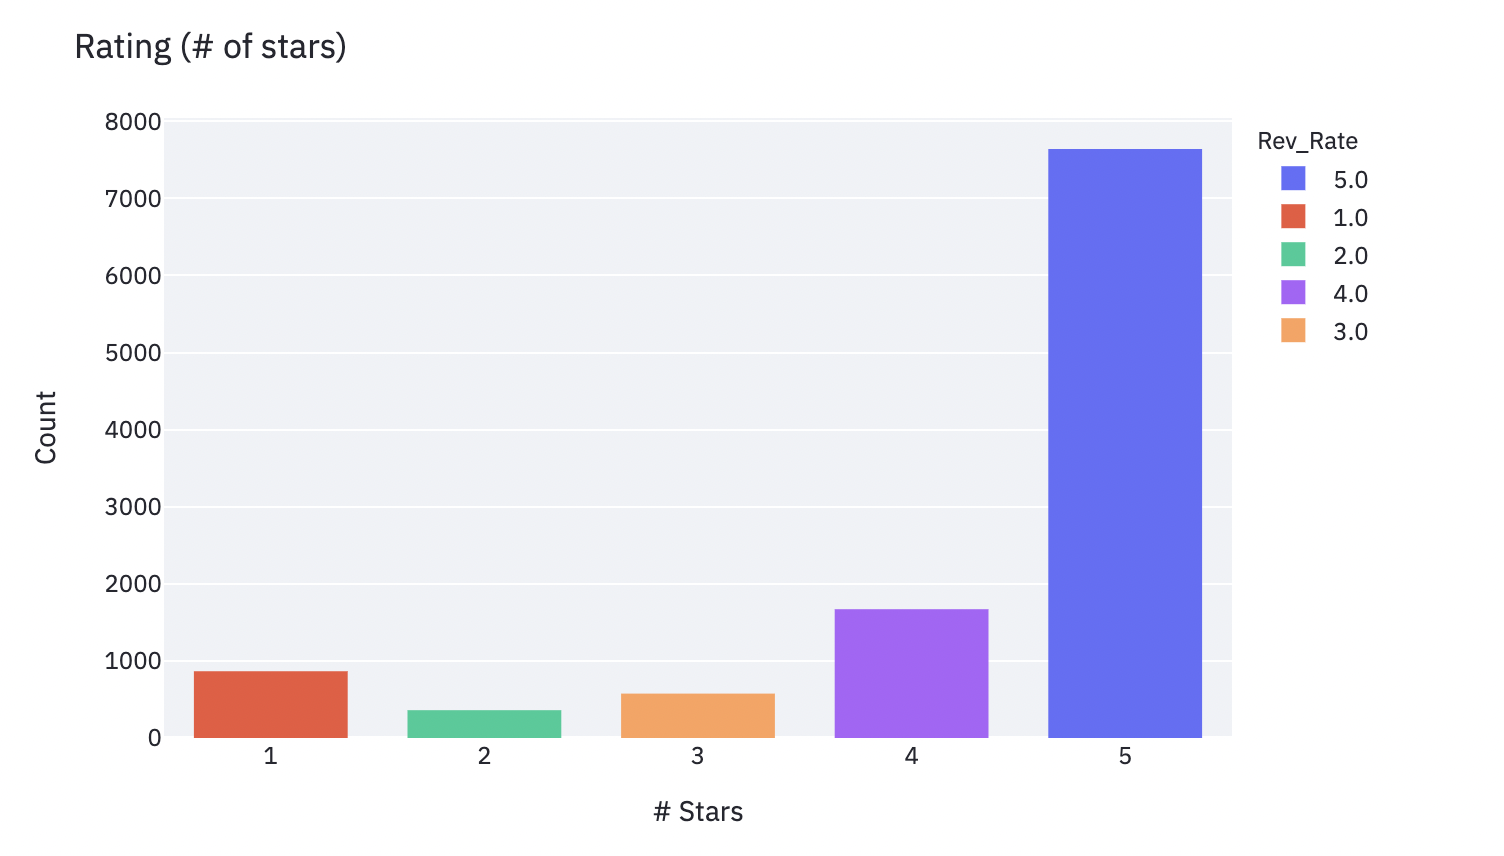
\includegraphics[scale=0.55]{src/img/rev_rate.png}
    \caption{Reviews Rating Distribution}
    \label{fig:my_label}
\end{figure}

\begin{figure}[H]
    \centering
    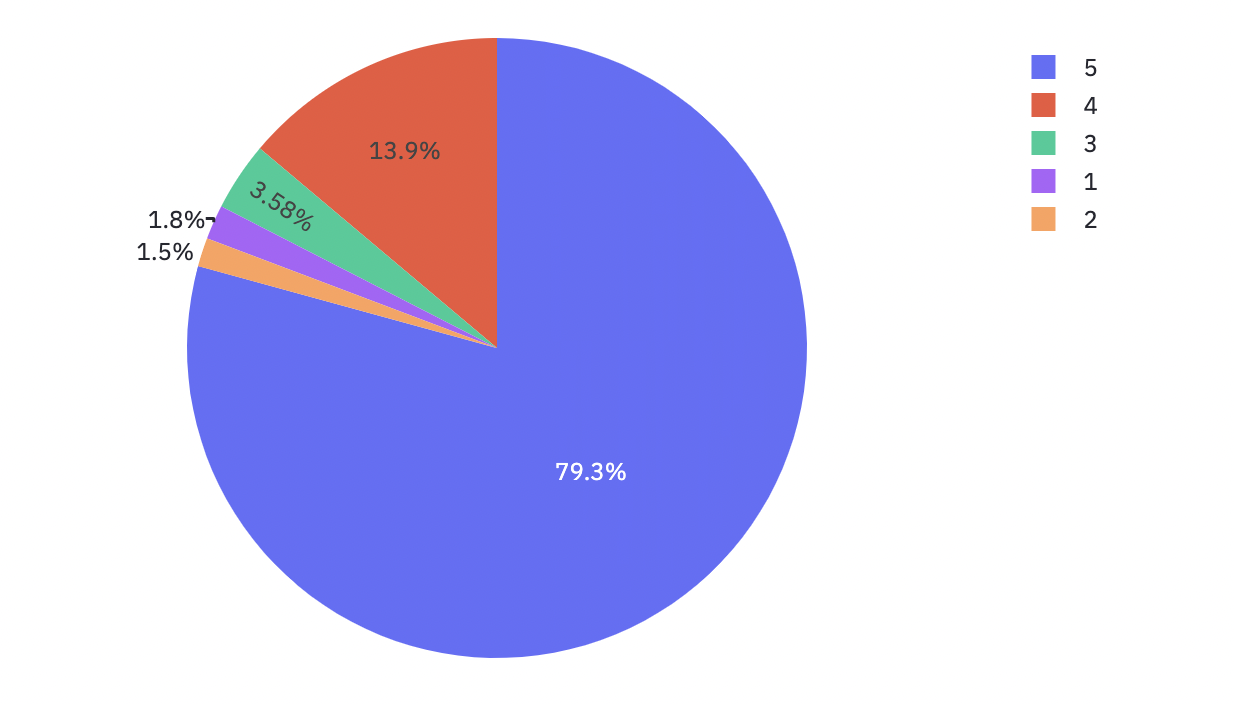
\includegraphics[scale=0.55]{src/img/rev_rate_pie.png}
    \caption{Reviews Rating Percentages}
    \label{fig:my_label}
\end{figure}

\subsubsection{ Which Classes got Highest Number of Reviews ? }
In this part of our project we are interested in analyzing sentiments of customers from their reviews\\
A possible solution is to calculate the number of reviews for our 3 classes and the following graph show that we have much more reviews with Positive Sentiment ( about 85\% from our data ) which is clearly dominating the two other classes, but it still logical from the previous ratings distribution where we got \textbf{4-5 stars} rating dominating.\\It is evident from the output that for almost all the reviews, the majority of the reviews are positive, followed by neutral and negative reviews.
\begin{figure}[H]
    \centering
    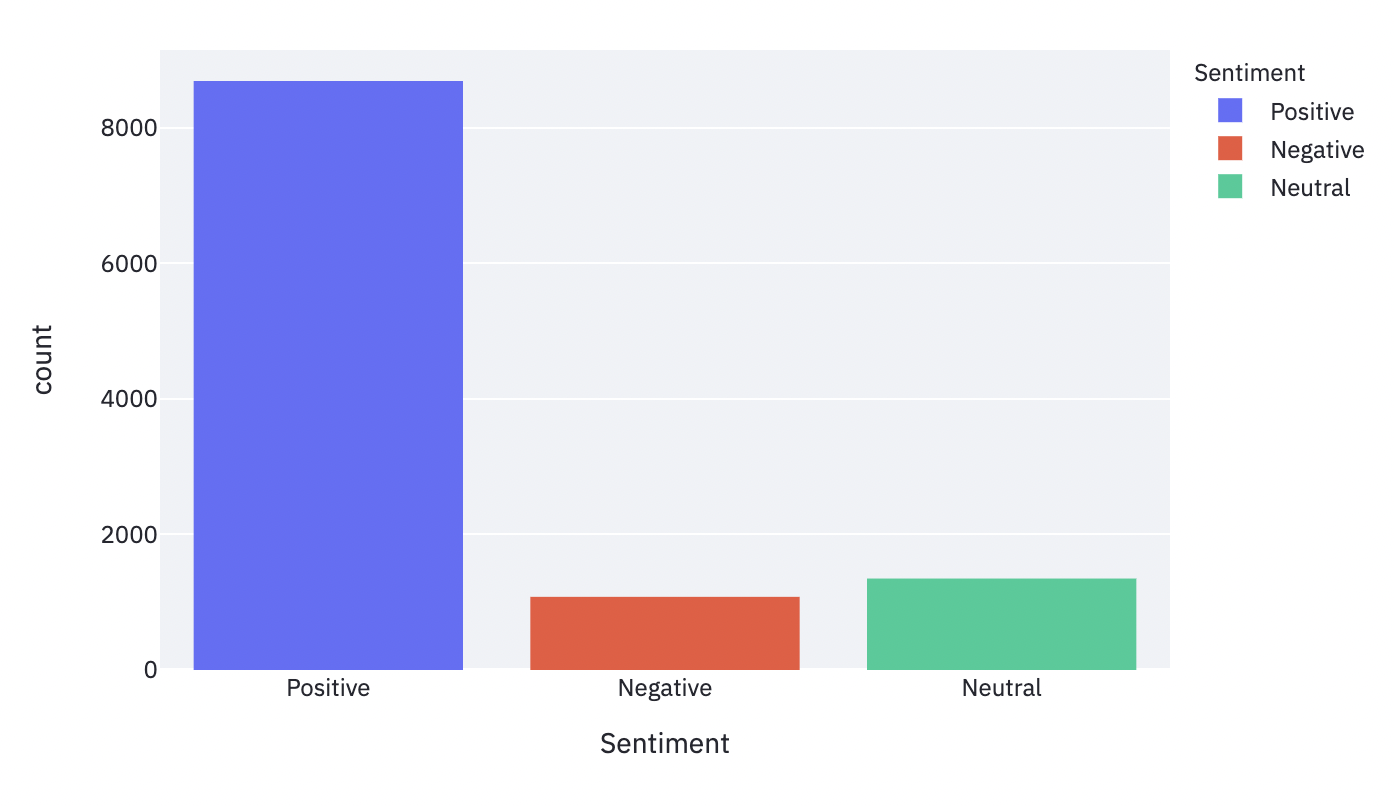
\includegraphics[scale=0.55]{src/img/classes.png}
    \caption{Reviews Sentiments Distribution}
    \label{fig:my_label}
\end{figure}
\textbf{Note.} The sentiment was generated based on \textbf{Polarity} attribute which we got from \mention{TextBlob-fr}

\subsubsection{How are Reviews Helpfulness in several products ? }
In this section of our project we are interested in analyzing how many people find other reviews helpful for the different products\\
Our data is categorized in \textbf{6} different categories
\textbf{(Informatique,Cuisine,Sports,Electromenager,Montres,Auto-moto)}\\
From the output, we can see that the product of ID 7 and 8 are the most helpful products and they are part of catgory \textbf{Cuisine}, but also the first category \textbf{Informatique} got many helpful tags on its reviews.\\
The last category compared to other ( in terms of helpfulness ) is \textbf{Auto-moto}.
\begin{figure}[H]
    \centering
    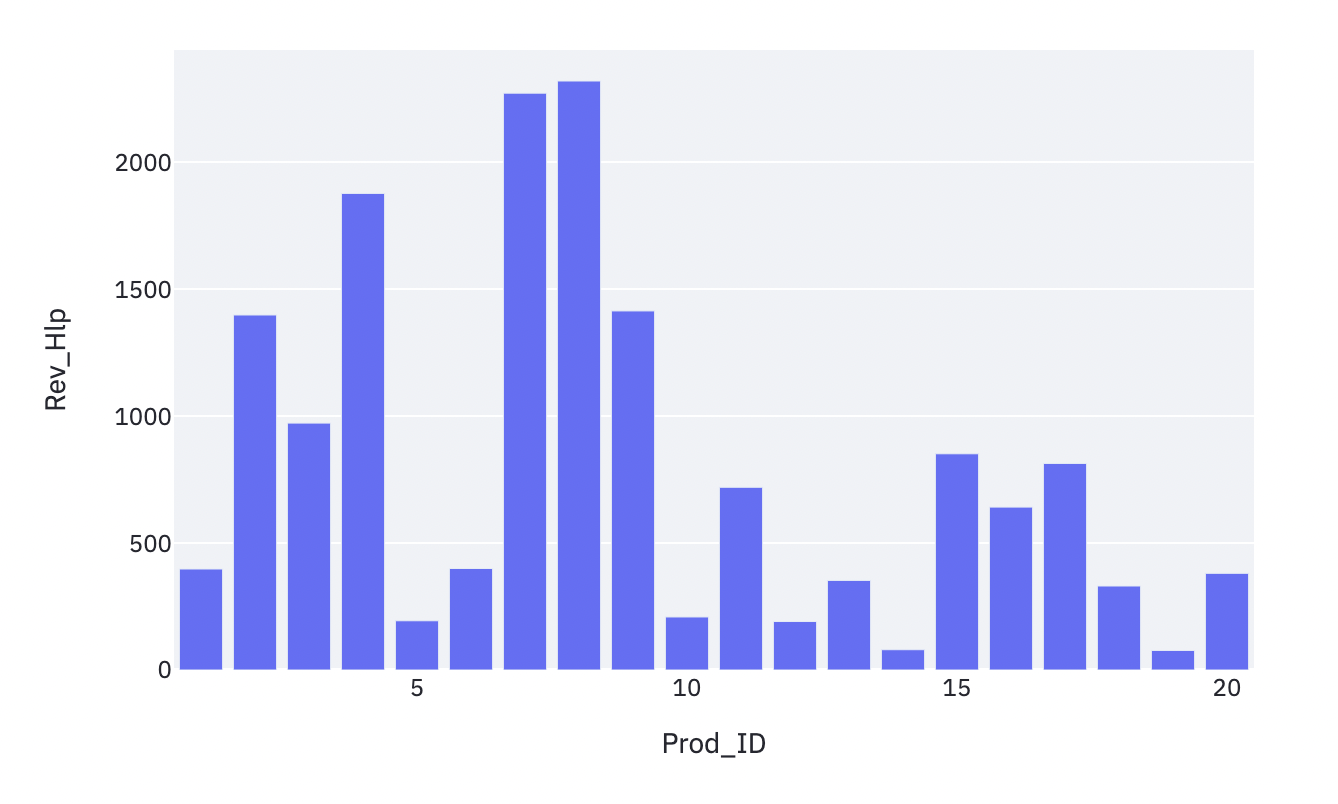
\includegraphics[scale=0.55]{src/img/prod_rev_hlp.png}
    \caption{Reviews Helpfulness Distribution}
    \label{fig:my_label}
\end{figure}
\textbf{Note.} We have respectively \textbf{4-4-2-4-4-2} products from the listed categories above.
\newpage
\subsubsection{How are Sentiments Distributed for the Reviews ? }
The $x$-axis shows polarity, and $y$-axis shows subjectivity.Polarity tells how positive or negative the text is. The subjectivity tells how subjective or opinionated the text is. The green dots that lies on the vertical line are the “neutral” reviews, the red dots on the left are the “negative” reviews, and the blue dots on the right are the “positive” reviews. Bigger dots indicate more subjectivity. We see that positive reviews are more than the negatives.
\begin{figure}[H]
    \centering
    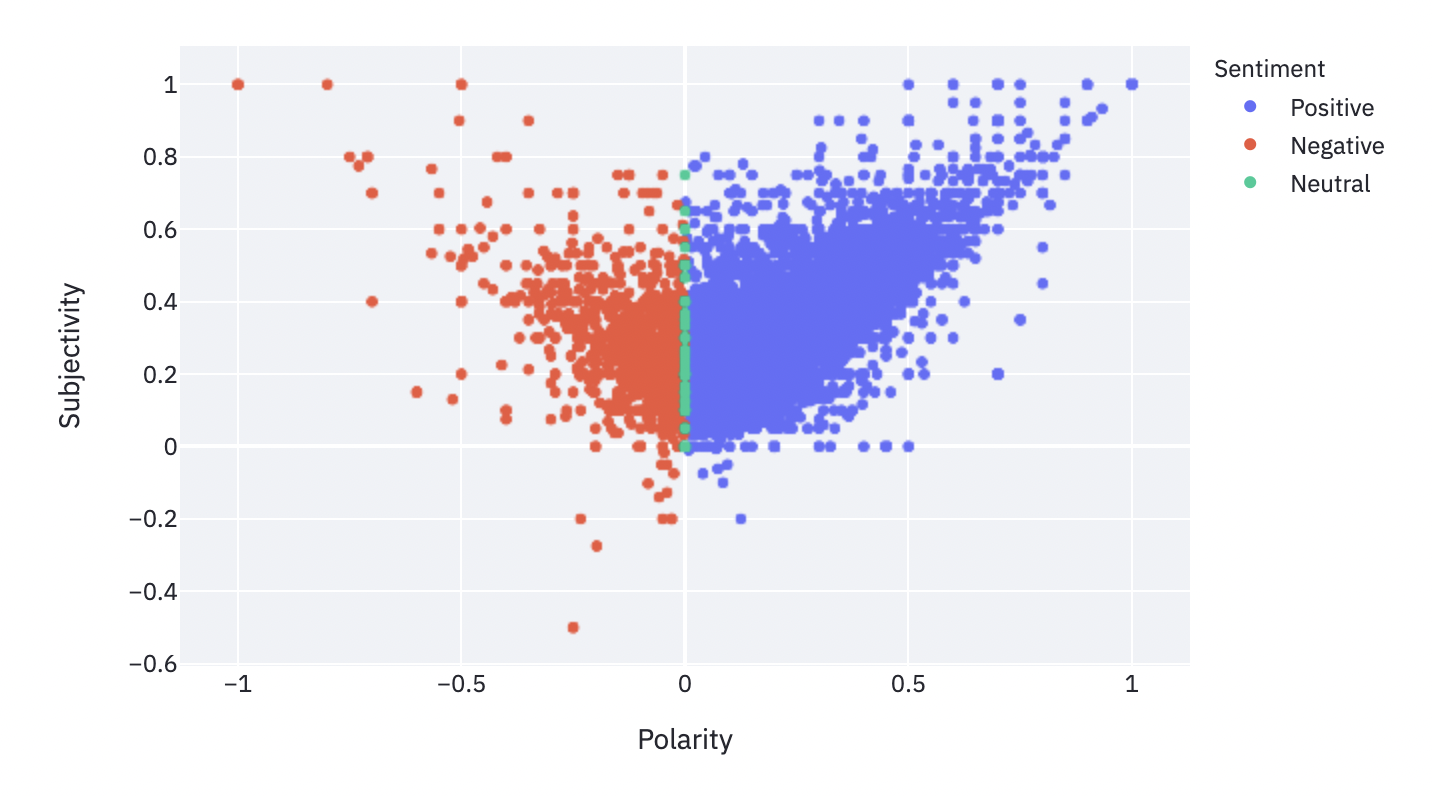
\includegraphics[scale=0.55]{src/img/polarity_subj_1.png}
    \caption{Reviews Sentiments Distribution}
    \label{fig:my_label}
\end{figure}

The same scatter graph can be represented in the following histogram in which we confirm the same information that positive comments are those who have a positive polarity and thet are much more than Neutral or Negative reviews which can bbe explained from the previous stats.\\
We also observe that this data is normally ditributed and between $0.7 - 0.8$ for Polarity we observe a higher value of subjectivity and from the meaning we can say that customers who react subjectivly on comment the have a higher probability to be with a positive sentiment and which completly logical.

\begin{figure}[H]
    \centering
    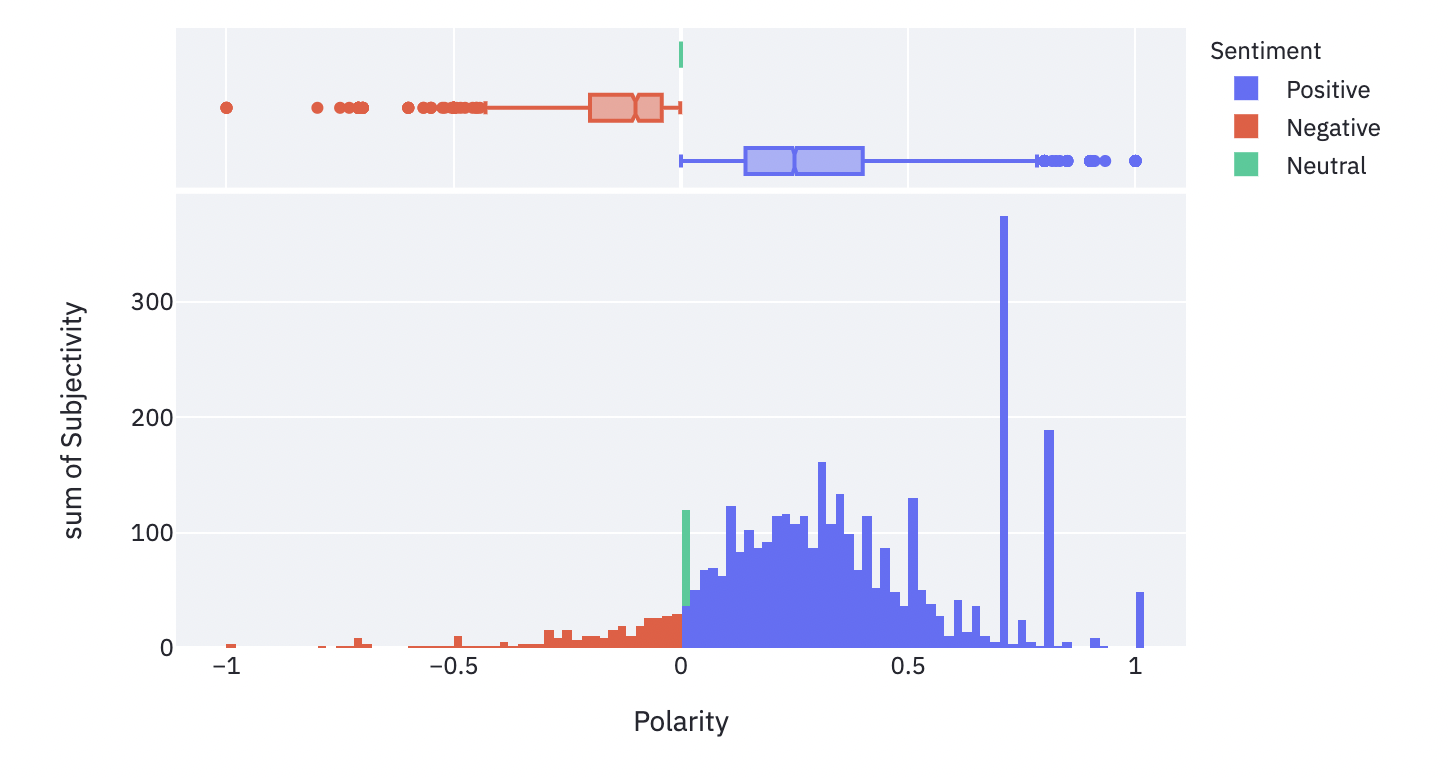
\includegraphics[scale=0.55]{src/img/polarity_subj_2.png}
    \caption{Reviews Snetiment Distribution}
    \label{fig:my_label}
\end{figure}

\newpage
\subsubsection{ Is there any relation between Stars Rating and Polarity ? }
In this part we are interested in the relation between polarity and number of stars in reviews rating , we can observe that for all stars ratings values polarity has more appearances between -0.25 and 0.25 and also as much as we have stars in review the polarity is higher which is what we expected and that show that no outliers are in our data, otherwise we would have ratings and Polarity in different order than what we got.
\begin{figure}[H]
    \centering
    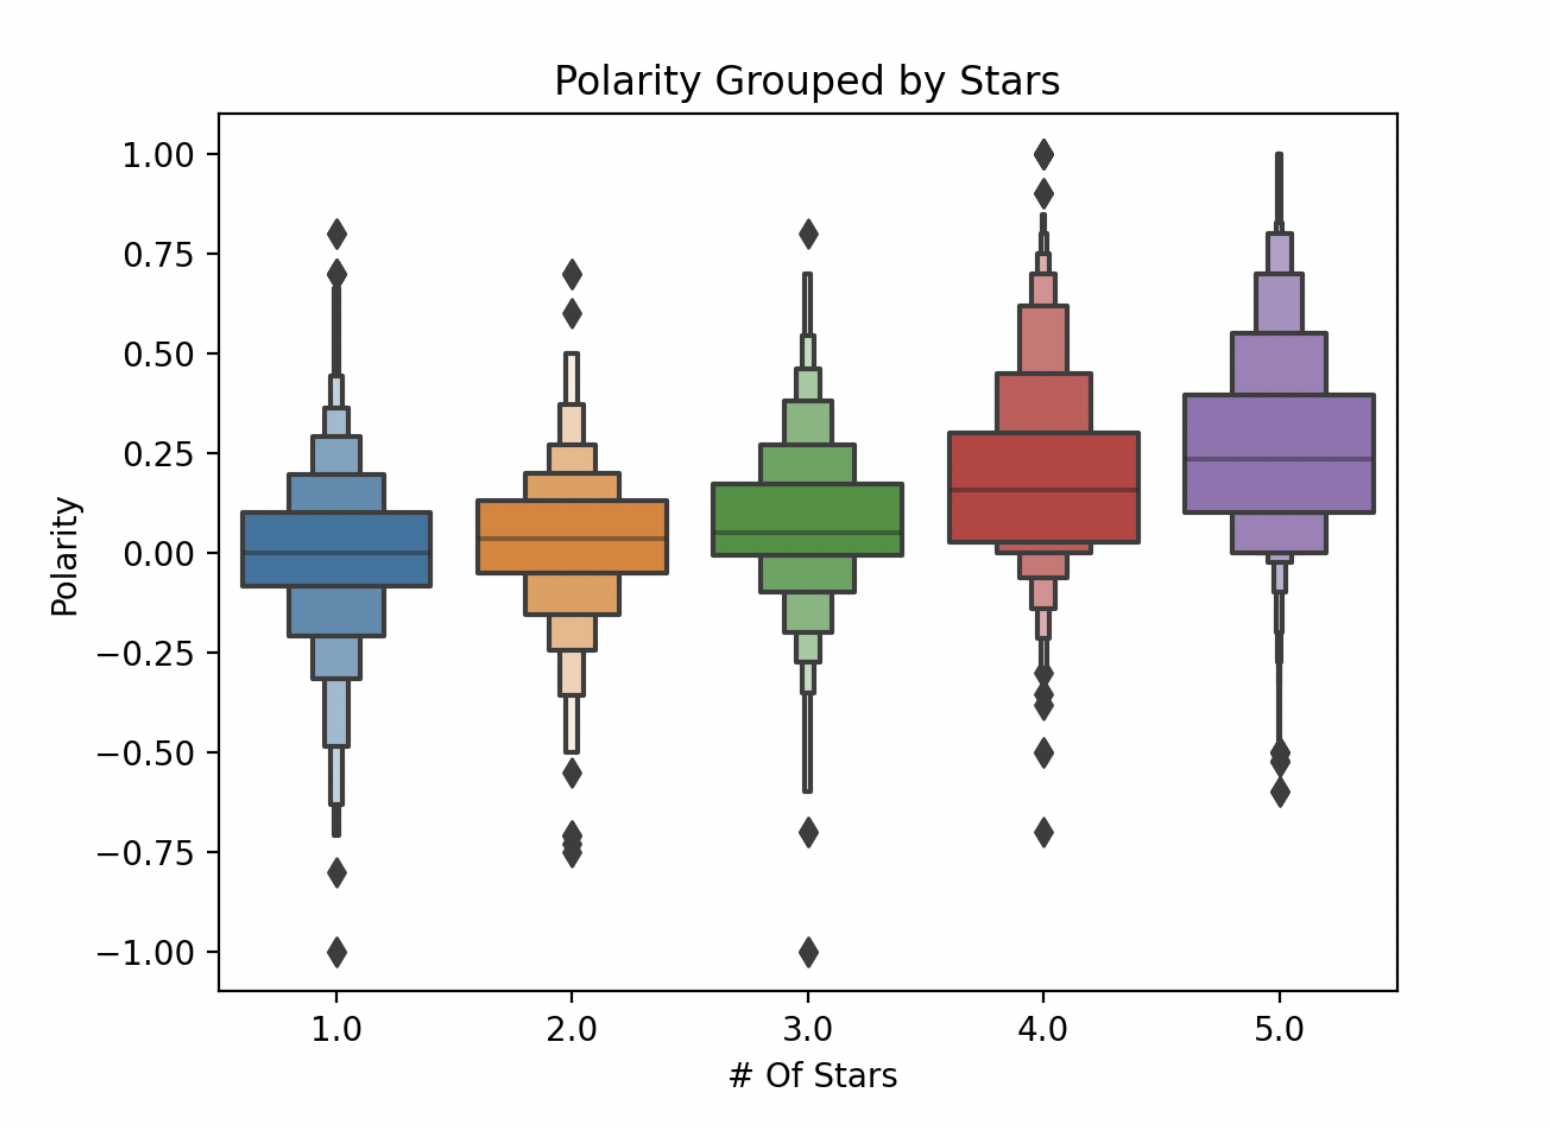
\includegraphics[scale=0.5]{src/img/Polarity_stars.png}
    \caption{Polarity Grouped By Stars Rating}
    \label{fig:my_label}
\end{figure}

\subsubsection{ Which words are used for Positve/Negative \& Neutral comments? }
We can see that there are some words which are repeated in both Positive and Neutral reviews which mean that In general customers are commenting with the same way (vocabulary) and we see that this step isn't that deducing because we cannot take any conclusion ( for example the word \mention{Bien} is present in the three classes which is confusing at the first sight ) but it can be explained with the fact of negation ( for example many people even with negative opinion can use this word but in a negative way ).
\begin{figure}[H]
    \centering
    \subfloat[\centering Positive Reviews]{{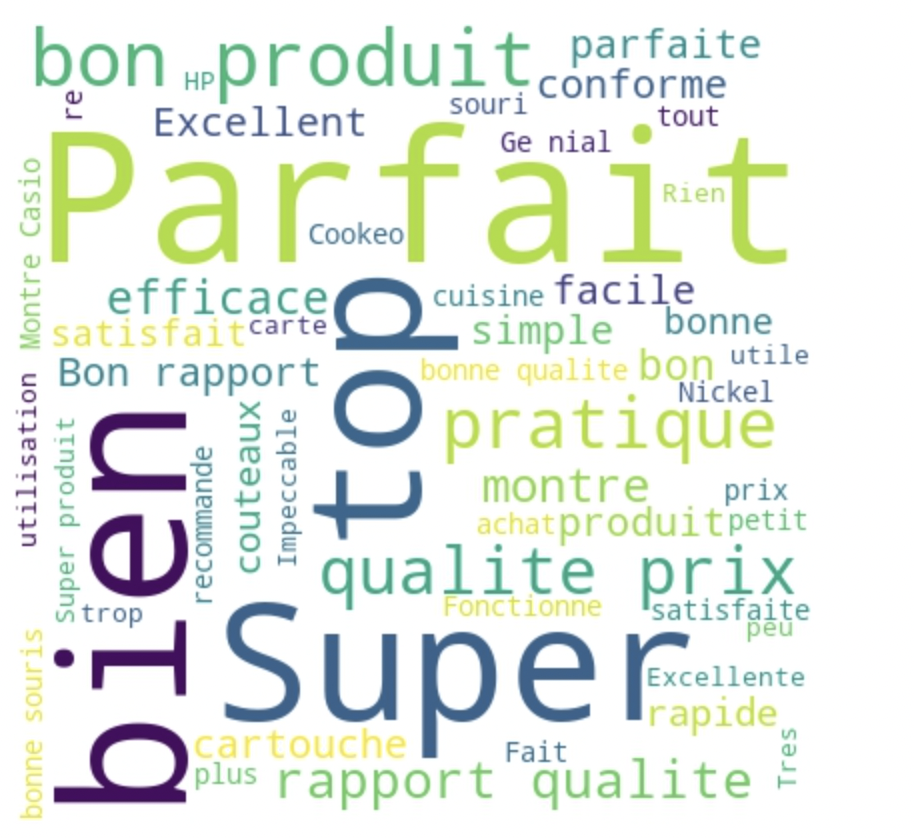
\includegraphics[width=5cm]{src/img/wc_pos.png} }}
    \qquad
    \subfloat[\centering Negative Reviews]{{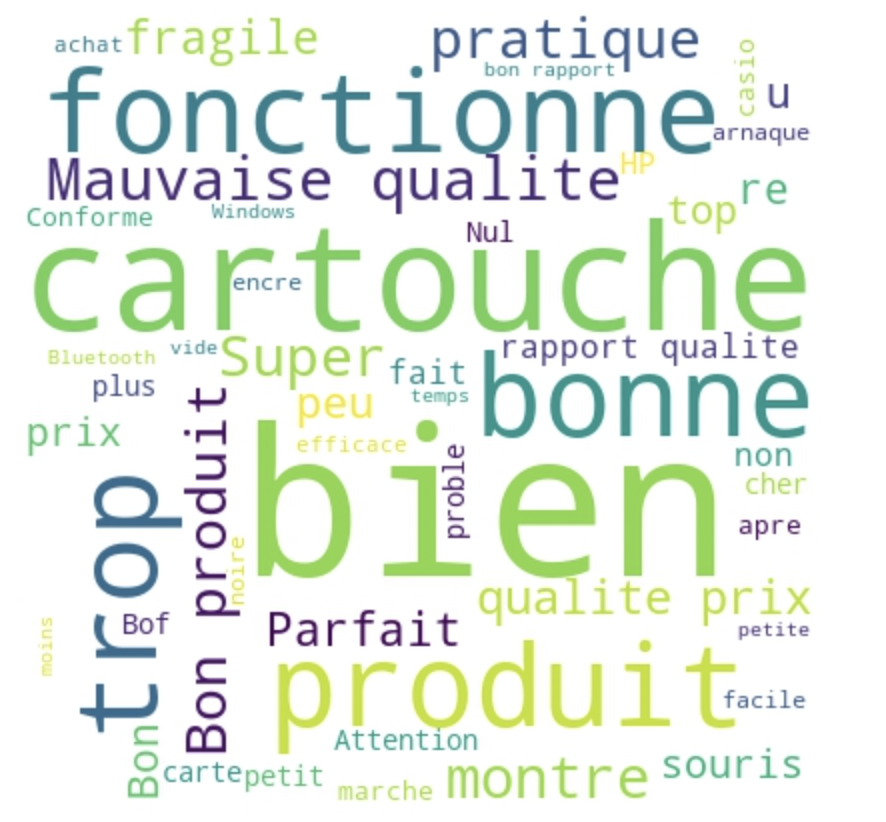
\includegraphics[width=5cm]{src/img/wc_neg.png} }}
    \subfloat[\centering Neutral Reviews]{{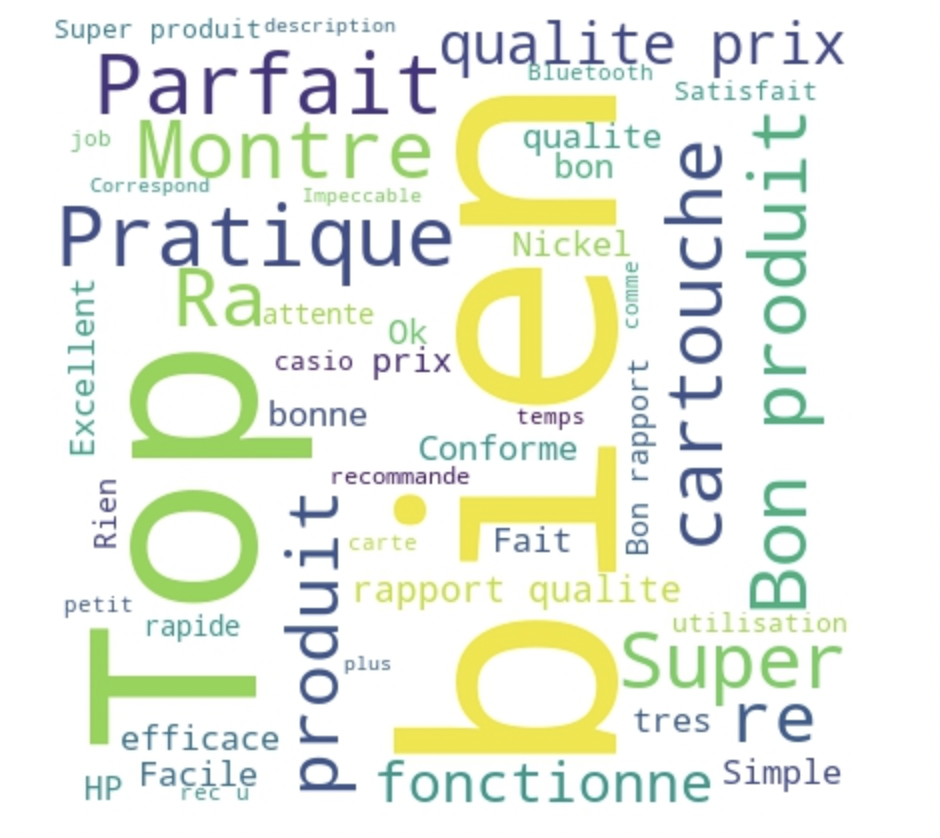
\includegraphics[width=5cm]{src/img/wc_neu.png} }}
    \qquad
    \caption{Word Clouds For Reviews by sentiment}
    \label{fig:example}
\end{figure}
\newpage
\section{ Machine Learning Models :  }
\subsection{Setting Classes to Reviews data : }
As we said in the beginning of our project , we have a task of classification with 3 classes , to get this classes we used the \mention{TextBlob-fr} Python's library to get a \mention{Sentiment} object which have as attributes \textbf{Polarity} and \textbf{Subjectivity}, the polarity will help us to set a class for a comment.This task is simply done with an encoder function as follow :
\begin{code}
def encode_sentiment(sentiment):
    if sentiment == 'Positive' :
      return 1
    elif sentiment == 'Negative' :
      return -1
    else :
      return 0

def decode_sentiment(data):
    if data > 0 :
      return 'Positive'
    elif data < 0 :
      return 'Negative'
    else :
      return 'Neutral'
\end{code}
\noindent
And so with this function we have the labels for our reviews.
\begin{code}
ds['Polarity'] = ds['Rev_Bdy'].apply(get_polarity)
ds['Sentiment'] = ds['Polarity'].apply(decode_sentiment)
y = ds['Sentiment'].apply(encode_sentiment)
\end{code}

\subsection{Dividing data into train and test sets : }
In the previous section, we converted the data into the numeric form. As the last step before we train our algorithms, we need to divide our data into training and testing sets. The training set will be used to train the algorithm while the test set will be used to evaluate the performance of the machine learning model.\\
Execute the following code:
\begin{code}
df = mx_rev.drop('Title',axis = 1)
X_train , X_test , y_train , y_test = train_test_split(df,y,test_size = 0.2)
\end{code}

\subsection{ Training Models :}
Once data is split into training and test set, machine learning algorithms can be used to learn from the training data. You can use any machine learning algorithm. However, we will use the SVM, KNN ($k$-Nearest Neighbors), Logistic Regression and Random Forest algorithms, owing to its ability to act upon non-normalized data.\\
We will use the help of \mention{Pipelines} to make the life easier !\\
To define any Model from the following we will use the following code :
\begin{code}
from sklearn.pipeline import Pipeline
model = Pipeline([
    ('vect', CountVectorizer()),
    ('tfidf', TfidfTransformer()),
    ('clf', Classifier()),
])
\end{code}
\newpage
\subsubsection{ SVM (Support Vector Machine):}
\paragraph{ Training SVM model : }
The sklearn.ensemble module contains the \mention{SVC} class that can be used to train the \textbf{SVM} Machine Learning model. To do so, we need to call the fit method on our pipeline  ( \mention{model} object ) the SVM class and pass it our training features and labels, as parameters.Look at the following script:
\begin{code}
from sklearn.pipeline import Pipeline

# Pipline of our model
model = Pipeline([
    ('vect', CountVectorizer()),
    ('tfidf', TfidfTransformer()),
    ('clf', SVC(params)),
])

# SVM params to be chosen
params = {
    'kernel' : ['poly','rbf'],
    'C' : [1,2,5,10,20,50,100,200,1000,2000,5000],
    'gamma' : [1e-1,1e-2,1e-3, 1e-4,1e-5],
    'degree' : [2,3],
    'decision_function_shape' : ['ovo','ovr'],

}
# GridSearchCV to get the best params
grid = GridSearchCV(model,param_grid = params, cv = 'number of folds for cross-validation' )

model.fit(X_train,y_train)
\end{code}

\textbf{Note .} the params object will be detailed in mode evaluation improvment via \mention{GridSearchCV} to get the best parameters

\paragraph{ Evaluating SVM model :}
Once the model has been trained, the last step is to make predictions on the model \\
Finally, to evaluate the performance of the machine learning models, we can use classification metrics such as a confusion metrix, F1 measure, accuracy, etc.
\begin{code}
from sklearn.metrics import confusion_matrix,accuracy_score,classification_report

y_pred = model.predict(X_test)

print(f'accuracy : {accuracy_score(y_pred, y_test)}')
print(classification_report(y_test, y_pred))

\end{code}
The output of the script above looks like this :
\begin{figure}[H]
    \centering
    \includegraphics[scale=0.55]{src/img/svm_score.png}
    \caption{SVM Evaluation}
    \label{fig:my_label}
\end{figure}
So As we saw we got 88\% accuracy using the \textbf{SVM} model we can show below the confusion matrix :
\begin{figure}[H]
    \centering
    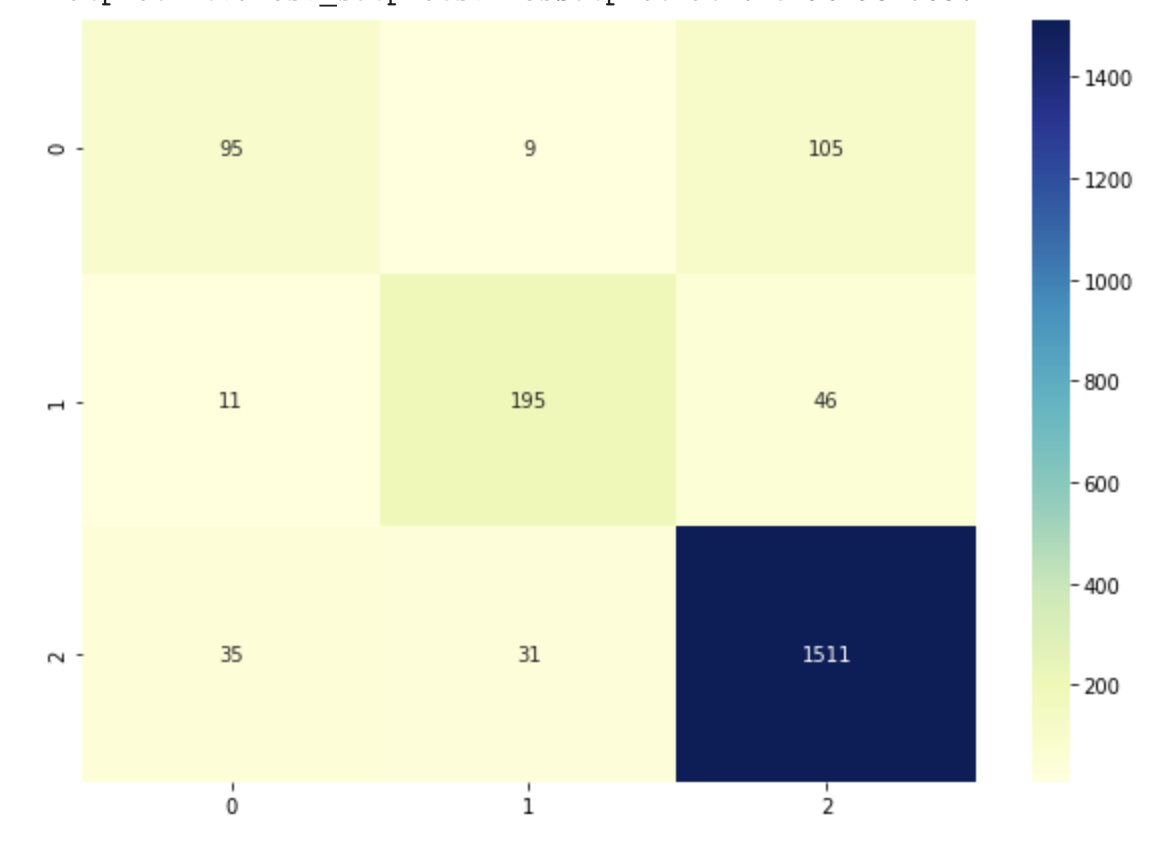
\includegraphics[scale=0.4]{src/img/svm_cm.png}
    \caption{SVM-evaluation Confusion Matrix}
    \label{fig:my_label}
\end{figure}
From what the confusion matrix and the classification report we can observe that the negative reviews are those which make the accuracy less than expected and that is expected beacause of the amount of negative reviews compared to the postive one's in our dataset.\\
We also tried to compare the performance of SVM models based on the hyperparmeter \textbf{C} and the kernel \textbf{rbf} and \textbf{linear} the following graph show that for values of \textbf{C} out of range  1..500 we have the same performance from rbf and linear kernels but inside this range we observe that the lineat kernel was better.\\
This doesn't mean that we should choose the \textbf{linear} kernel, because when searching for the best parameters using the \mention{GridSearchCv} we got that the best value for \textbf{C = 1000} which clearly out of the range of dominance that linear kernel show us.
\begin{figure}[H]
    \centering
    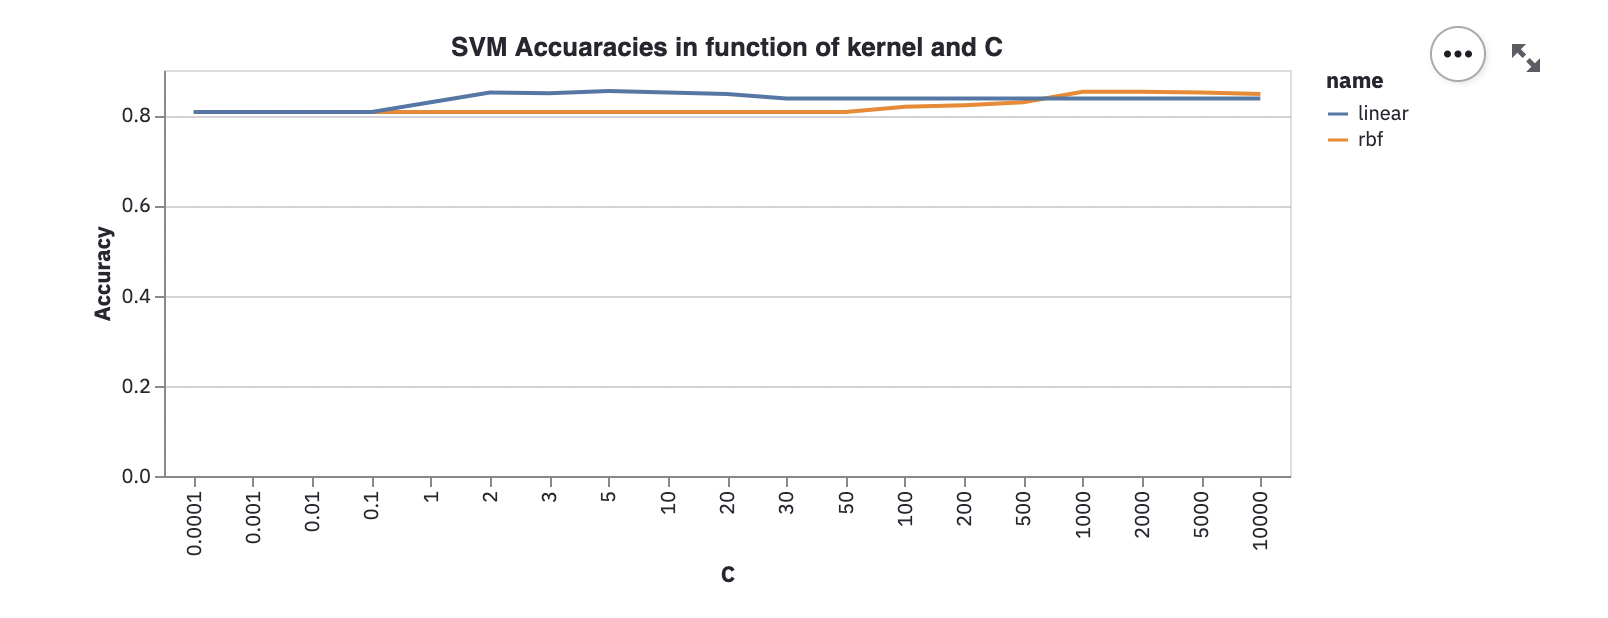
\includegraphics[scale=0.65]{src/img/svm_stats.png}
    \caption{SVM-evaluation Kernel stats}
    \label{fig:my_label}
\end{figure}
\textbf{Note .}
The process of grid search consumed a lot of time because it constructs multiple models for all possible combinations of param values in the param\_grid dictionary. So, here we are only tuning two parameters: C and kernel.

\newpage
\subsubsection{ $k$-NN ($k$-Nearest Neighbors):}
\paragraph{ Training KNN model : }
The sklearn.ensemble module contains the \mention{KNeighborsClassifier} class that can be used to train the \textbf{KNN} Machine Learning model. To do so, we need to call the fit method on our pipeline  ( \mention{model} object ) the KNeighborsClassifier class and pass it our training features and labels, as parameters.Look at the following script:
\begin{code}
# KNN params to be chosen
params = {
    'n_neighbors' : [range(1,21)],
    'weights' : ['uniform','distance'],
    'metric' : ['minkowski','manhattan','euclidean','cosine'],
}

# GridSearchCV to get the best params
model = GridSearchCV(model,param_grid = params, cv = 'number of folds for cross-validation')

model.fit(X_train,y_train)
\end{code}

\textbf{Note .} the params object will be detailed in mode evaluation improvment via \mention{GridSearchCV} to get the best parameters

\paragraph{ Evaluating KNN model :}
Once the model has been trained, the last step is to make predictions on the model \\
Finally, to evaluate the performance of the machine learning models, we can use classification metrics such as a confusion metrix, F1 measure, accuracy, etc.
\begin{code}
from sklearn.metrics import confusion_matrix,accuracy_score,classification_report

y_pred = model.predict(X_test)

print(f'accuracy : {accuracy_score(y_pred, y_test)}')
print(classification_report(y_test, y_pred))

\end{code}
The output of the script above looks like this :
\begin{figure}[H]
    \centering
    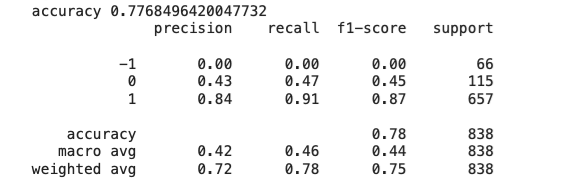
\includegraphics[scale=0.55]{src/img/knn_acc.png}
    \caption{KNN Evaluation}
    \label{fig:my_label}
\end{figure}
So As we saw we got 77\% accuracy using the \textbf{KNN} model we can show below the confusion matrix :
\begin{figure}[H]
    \centering
    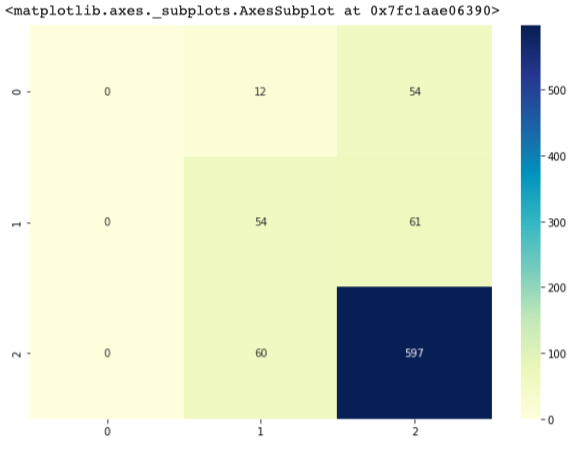
\includegraphics[scale=0.4]{src/img/knn_cm.png}
    \caption{KNN-evaluation Confusion Matrix}
    \label{fig:my_label}
\end{figure}
From what the confusion matrix and the classification report we can observe that the negative reviews are those which make the accuracy less than expected and that is expected because of the amount of negative reviews compared to the positive one's in our dataset.\\
We also tried to compare the performance of KNN models based on the hyperparmeter \textbf{n\_neighbors} the following graph show that for values of \textbf{n\_neighbors} bigger than 15 are the best for the accuracy but we also observe that they are mostly in constant variation which means there is no need to increase more this parameter than 15.\\
\begin{figure}[H]
    \centering
    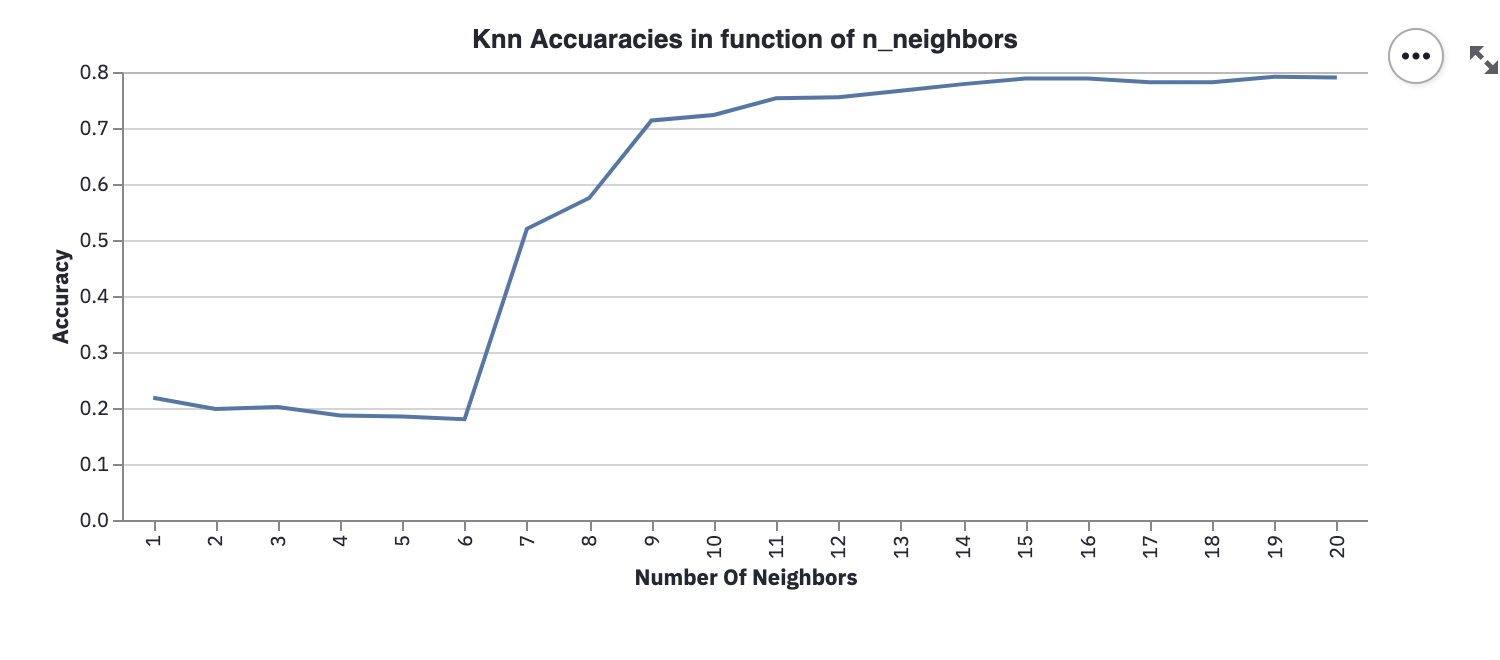
\includegraphics[scale=0.4]{src/img/knn_accuracies.png}
    \caption{KNN-evaluation neighbors stats}
    \label{fig:my_label}
\end{figure}
\newpage
\subsubsection{ Logistic Regression Model :}
\paragraph{ Training Logistic Regression model : }
The sklearn.ensemble module contains the \mention{LogisticRegression} class that can be used to train the \textbf{LogisticRegression} Machine Learning model. To do so, we need to call the fit method on our pipeline  ( \mention{model} object ) the LogisticRegression class and pass it our training features and labels, as parameters.Look at the following script:
\begin{code}
# LogisticRegression params to be chosen
params = {
    'C' : [1,2,5,10,20,50,100,200,1000,2000,5000],
    'tol' : np.linespace(0,1,200),
    'penalty' : ['l1','l2','none'],
}

# GridSearchCV to get the best params
grid = GridSearchCV(model,param_grid = params, cv = '# of folds for cross-validation')

model.fit(X_train,y_train)
\end{code}

\textbf{Note .} the params object will be detailed in mode evaluation improvment via \mention{GridSearchCV} to get the best parameters

\paragraph{ Evaluating Logistic Regression model :}
Once the model has been trained, the last step is to make predictions on the model \\
Finally, to evaluate the performance of the machine learning models, we can use classification metrics such as a confusion metrix, F1 measure, accuracy, etc.
\begin{code}
from sklearn.metrics import confusion_matrix,accuracy_score,classification_report

y_pred = model.predict(X_test)

print(f'accuracy : {accuracy_score(y_pred, y_test)}')
print(classification_report(y_test, y_pred))

\end{code}
The output of the script above looks like this :
\begin{figure}[H]
    \centering
    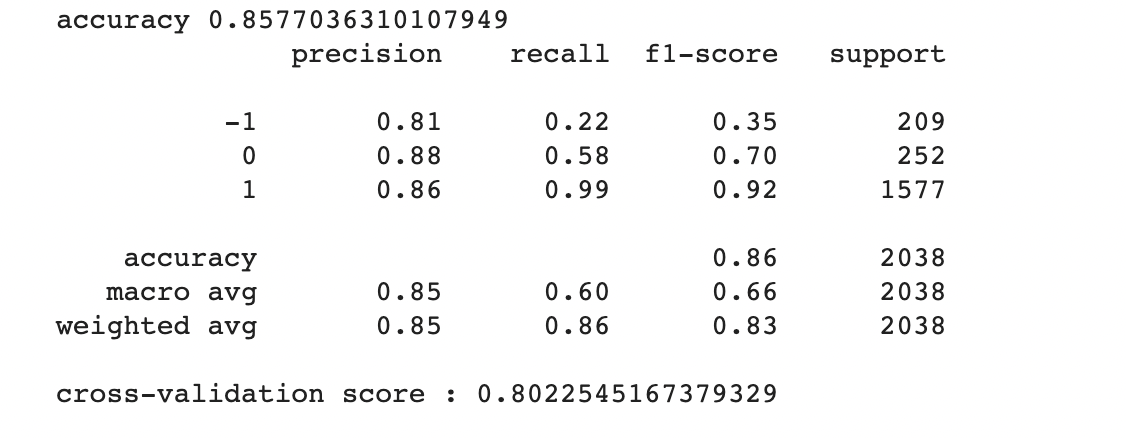
\includegraphics[scale=0.55]{src/img/log_reg_acc.png}
    \caption{Logistic Regression Evaluation}
    \label{fig:my_label}
\end{figure}
So As we saw we got 85\% accuracy using the \textbf{Logistic Regression} model we can show below the confusion matrix :
\begin{figure}[H]
    \centering
    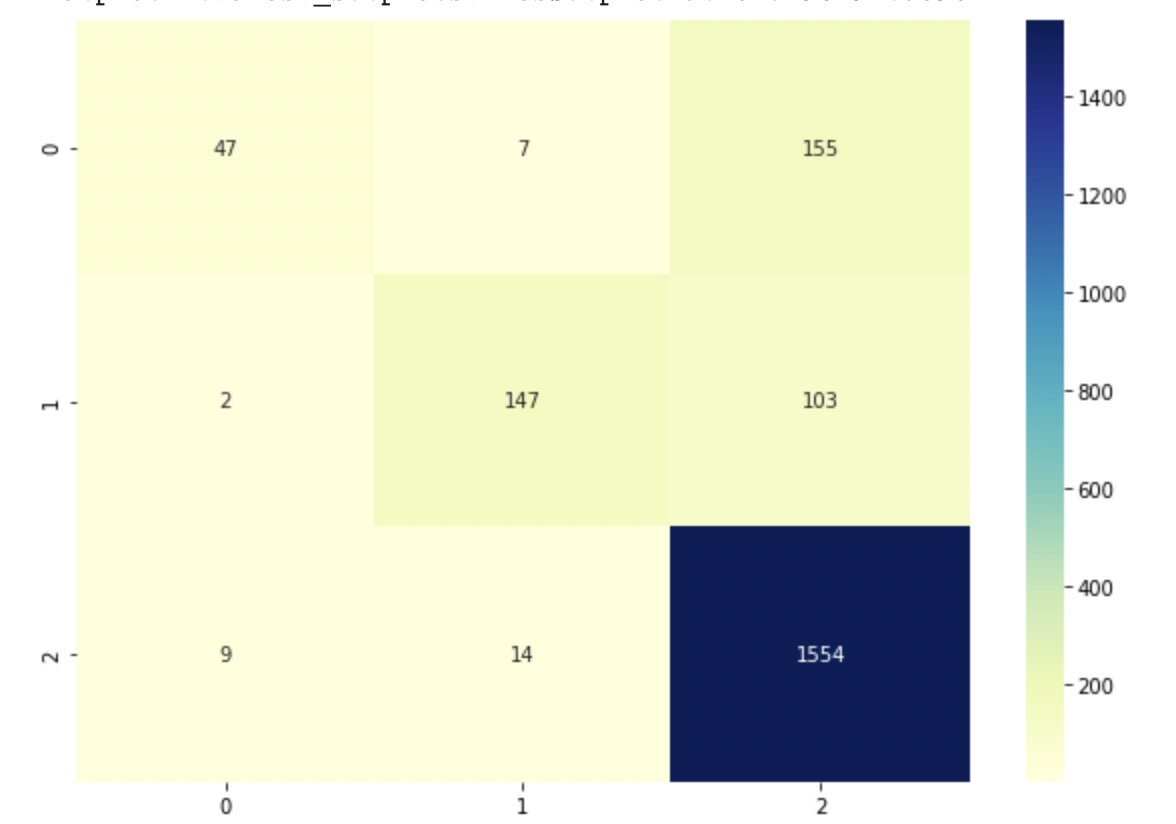
\includegraphics[scale=0.4]{src/img/log_reg_cm.png}
    \caption{Logistic Regression-evaluation Confusion Matrix}
    \label{fig:my_label}
\end{figure}
From what the confusion matrix and the classification report we can observe that the negative reviews are those which make the accuracy less than expected and that is expected because of the amount of negative reviews compared to the positive one's in our dataset.\\
So basically the same issue is present in all trained models which is the amount of negative reviews

\newpage
\subsubsection{ Random Forest Model:}
\paragraph{ Training RandomForest model : }
The sklearn.ensemble module contains the \mention{RandomForestClassifier} class that can be used to train the \textbf{RandomForestClassifier} Machine Learning model. To do so, we need to call the fit method on our pipeline  ( \mention{model} object ) the RandomForestClassifier class and pass it our training features and labels, as parameters.Look at the following script:
\begin{code}
# RandomForestClassifier params to be chosen
params = {
    'n_estimators': [100, 300, 500, 800, 1200],
    'max_features': ['auto', 'sqrt', 'log2'],
    'max_depth' : [4,5,6,7,8,15,25,30],
    'criterion' :['gini', 'entropy'],
    'min_samples_leaf' : [1, 2, 5, 10],
    'min_samples_split' : [2, 5, 10, 15, 100]
}

# GridSearchCV to get the best params
grid = GridSearchCV(model,param_grid = params, cv = '# of folds for cross-validation')

model.fit(X_train,y_train)
\end{code}

\textbf{Note .} the params object will be detailed in mode evaluation improvment via \mention{GridSearchCV} to get the best parameters

\paragraph{ Evaluating RandomForest model :}
Once the model has been trained, the last step is to make predictions on the model \\
Finally, to evaluate the performance of the machine learning models, we can use classification metrics such as a confusion metrix, F1 measure, accuracy, etc.
\begin{code}
from sklearn.metrics import confusion_matrix,accuracy_score,classification_report

y_pred = model.predict(X_test)

print(f'accuracy : {accuracy_score(y_pred, y_test)}')
print(classification_report(y_test, y_pred))

\end{code}
The output of the script above looks like this :
\begin{figure}[H]
    \centering
    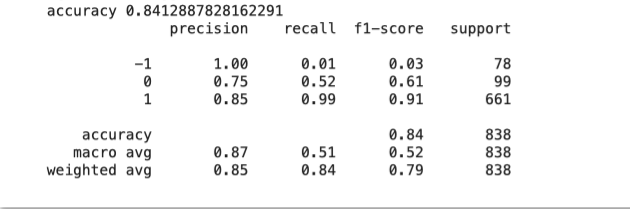
\includegraphics[scale=0.55]{src/img/rand_acc.png}
    \caption{RandomForest Evaluation}
    \label{fig:my_label}
\end{figure}
So As we saw we got 84\% accuracy using the \textbf{RandomForest} model we can show below the confusion matrix :
\begin{figure}[H]
    \centering
    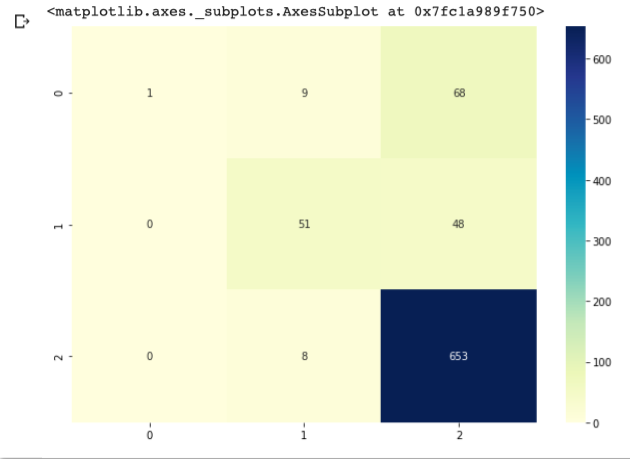
\includegraphics[scale=0.4]{src/img/rand_cm.png}
    \caption{RandomForest-evaluation Confusion Matrix}
    \label{fig:my_label}
\end{figure}
From what the confusion matrix and the classification report we can observe now another results which are slightly different from the first 3 models , here we have much less errors in precision for the negative reviews which is expected because of the work of a RandomForest and as known RandomForest can do much better but the computations will be more expensive in terms of cpu and time.

\section{Wanna Compare the performance of these models ?}
Yes ! , we have a solution for you. We decided to develop a Python web-application using the \mention{Streamlit} API so it make it simple and friendly to train the model you want on our dataset and change the parameters as you want.\\
We also managed to represent the dataset firstly and after cleaning and also all EDA's are there ! \\
Here some screenshots , and don't hesitate to test out this awesome application !
\begin{figure}[H]
    \centering
    \subfloat[\centering]{{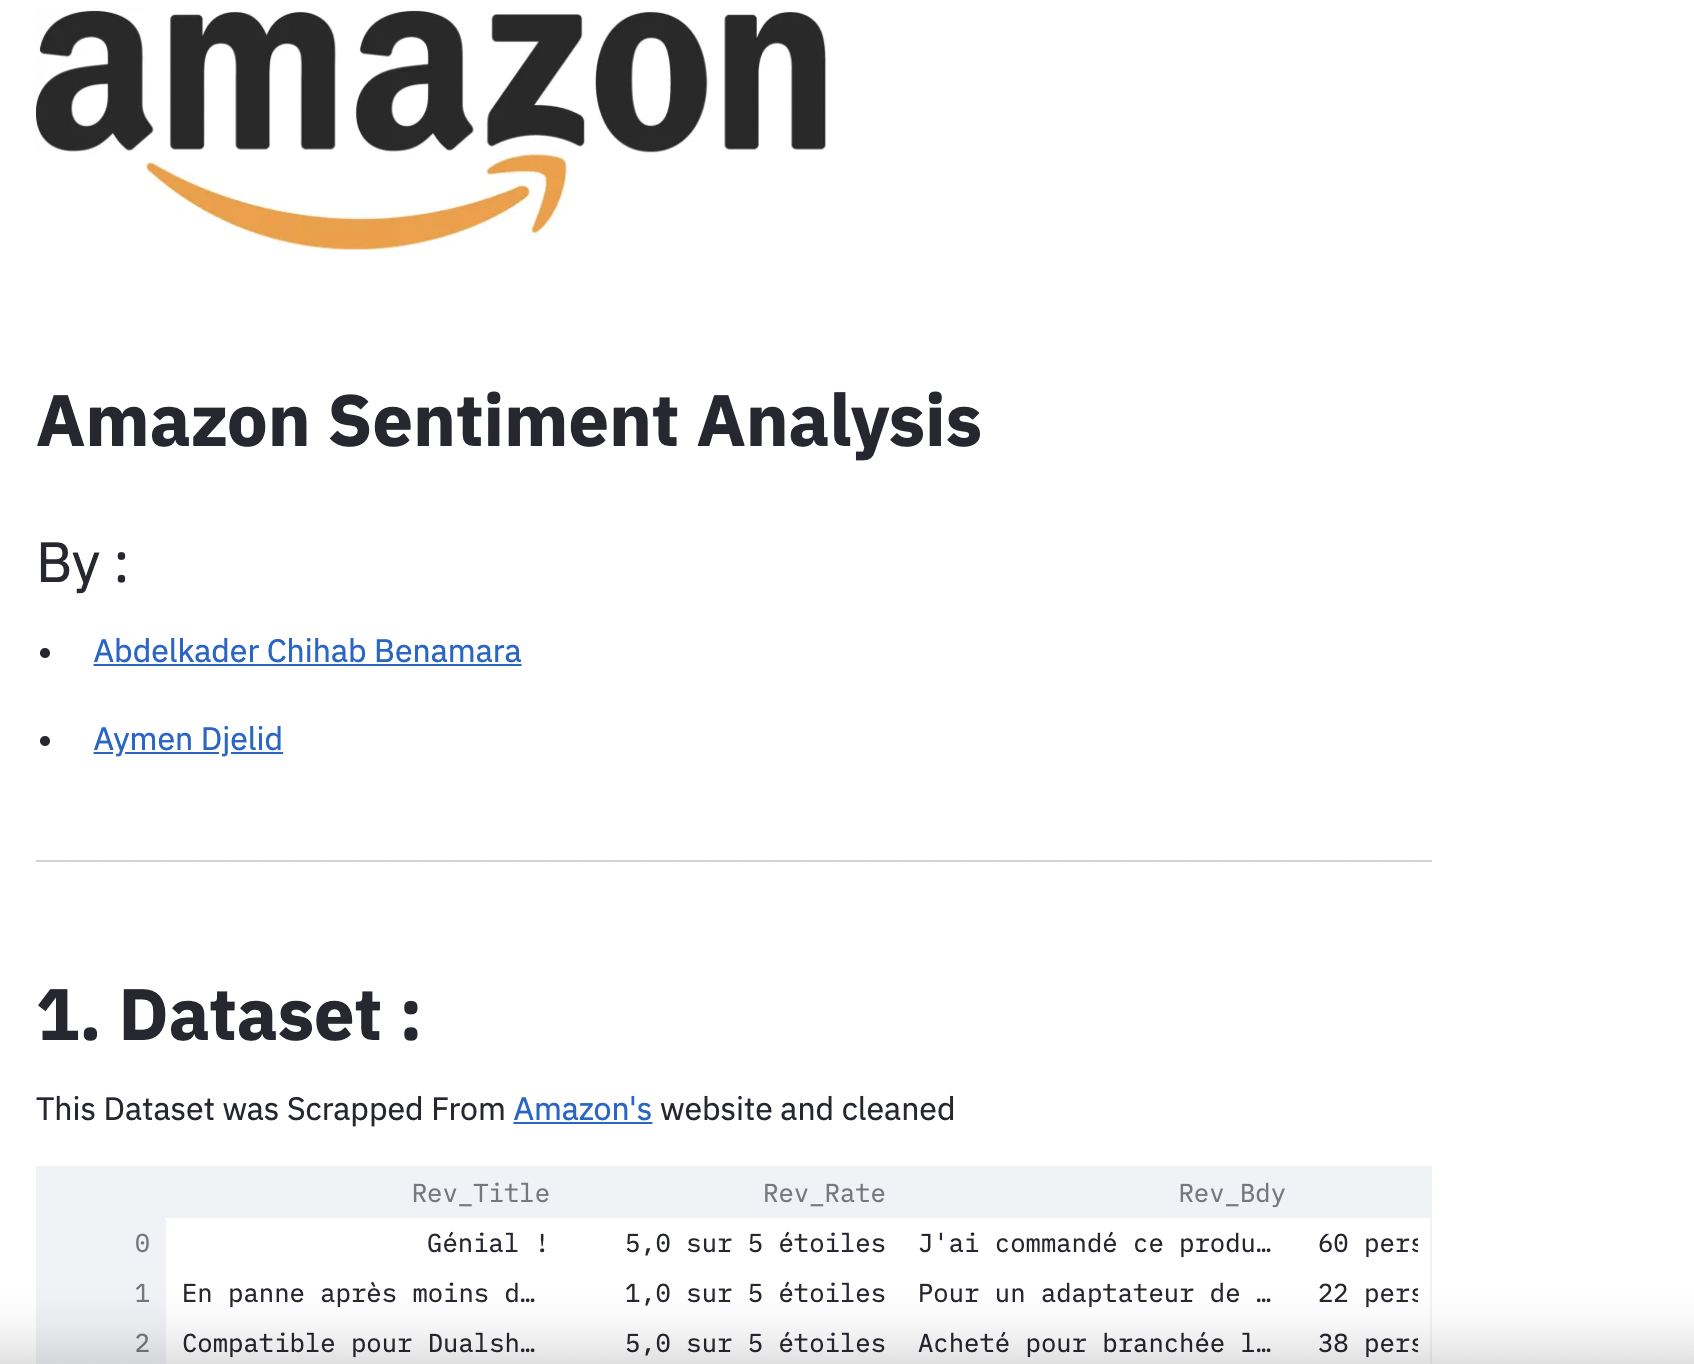
\includegraphics[width=8cm]{src/img/app_1.png} }}
    \qquad
    \subfloat[\centering]{{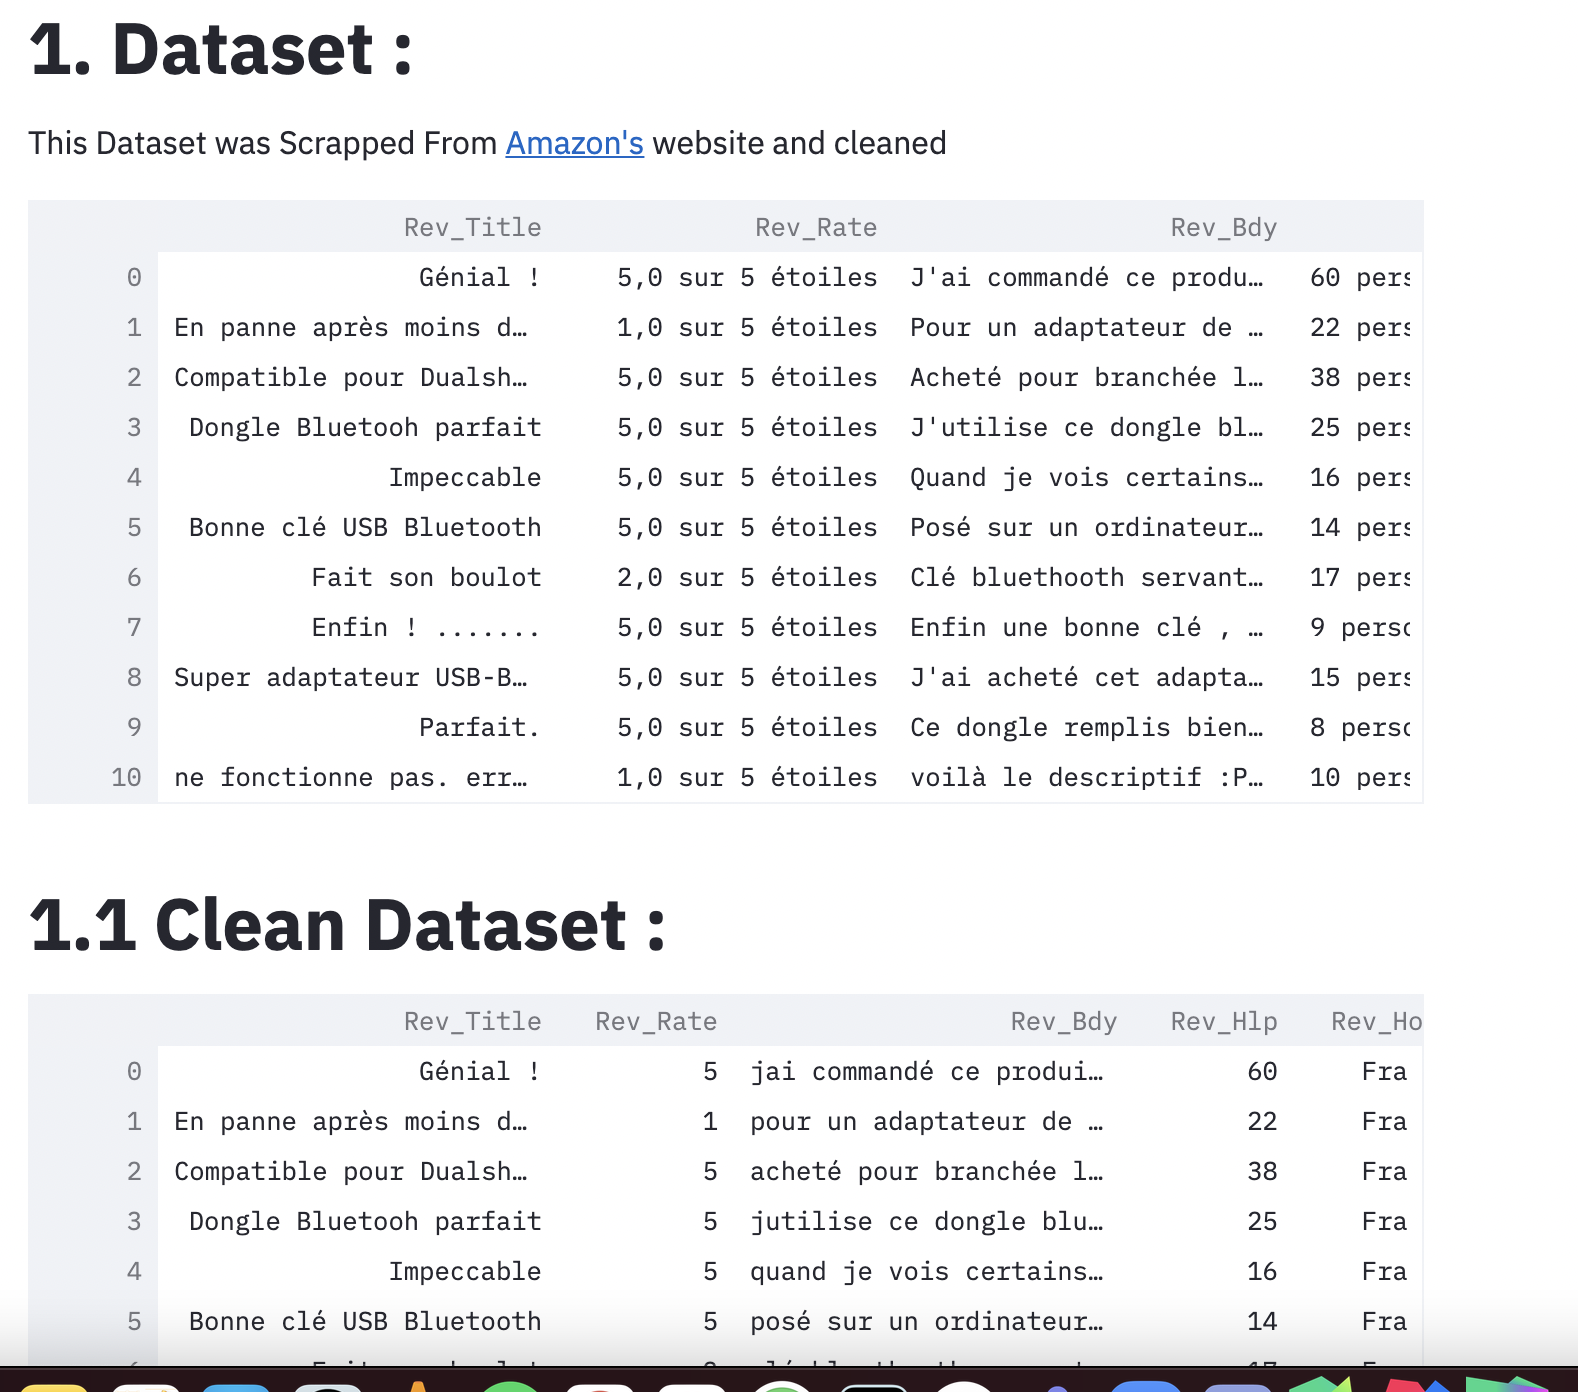
\includegraphics[width=8cm]{src/img/app_2.png} }}
    \caption{Some Screenshot from our website}
    \label{fig:example}
\end{figure}
\begin{figure}[H]
    \centering
    \subfloat[\centering]{{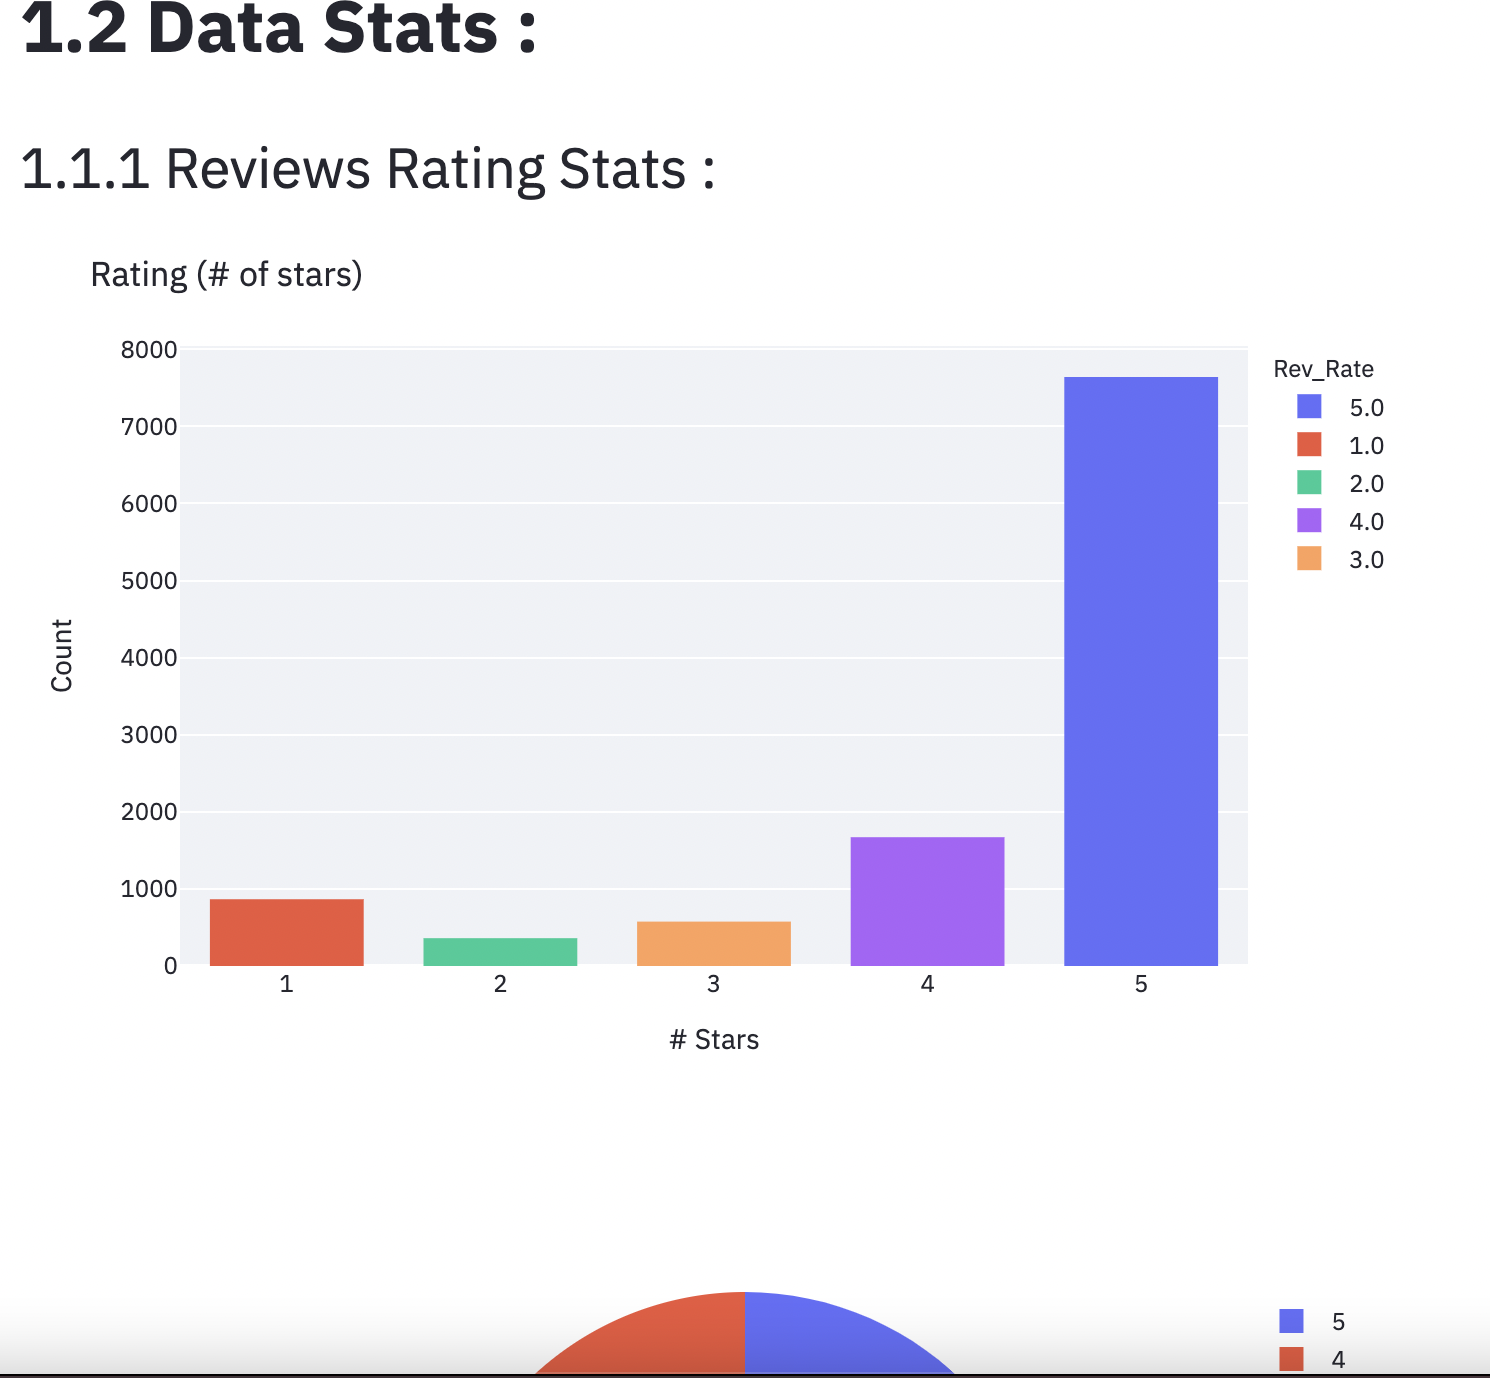
\includegraphics[width=8cm]{src/img/app_3.png} }}
    \qquad
    \subfloat[\centering]{{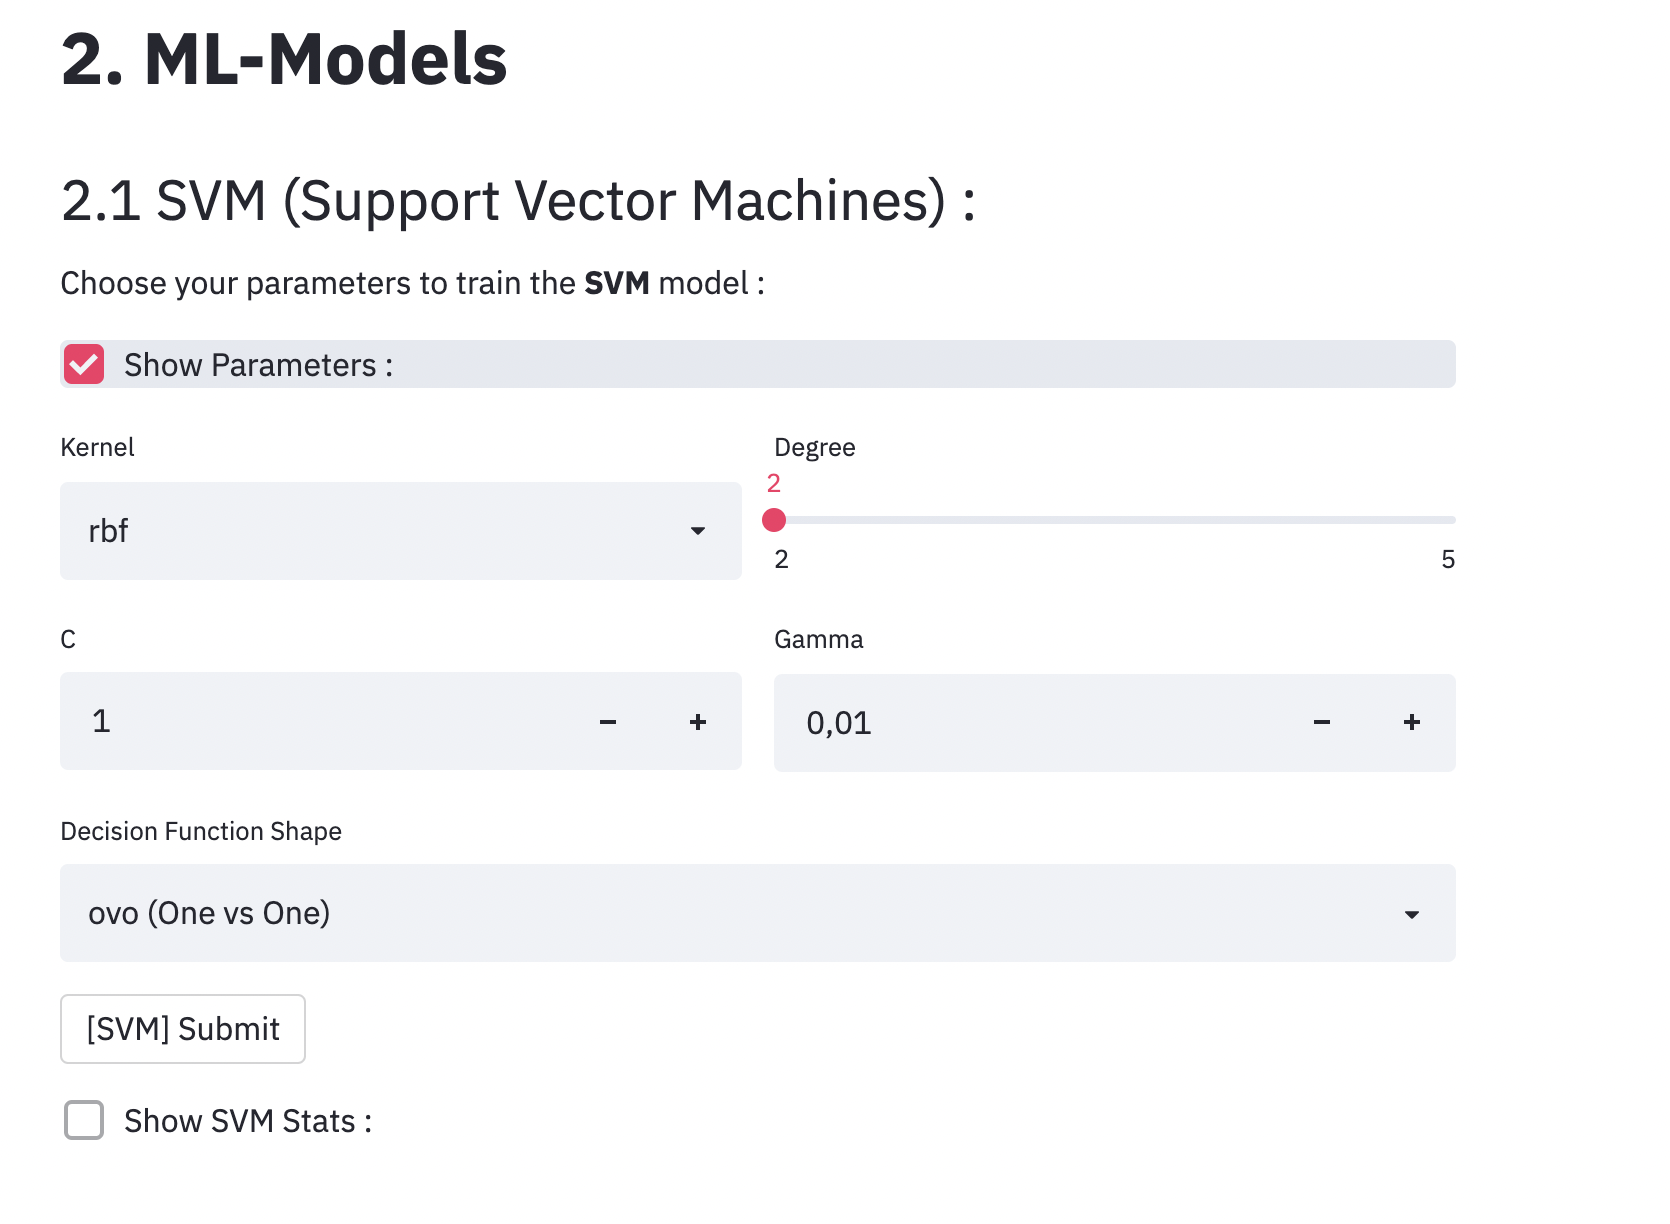
\includegraphics[width=8cm]{src/img/app_4.png} }}
    \caption{Some Screenshot from our website}
    \label{fig:example}
\end{figure}
\begin{figure}[H]
    \centering
    \subfloat[\centering]{{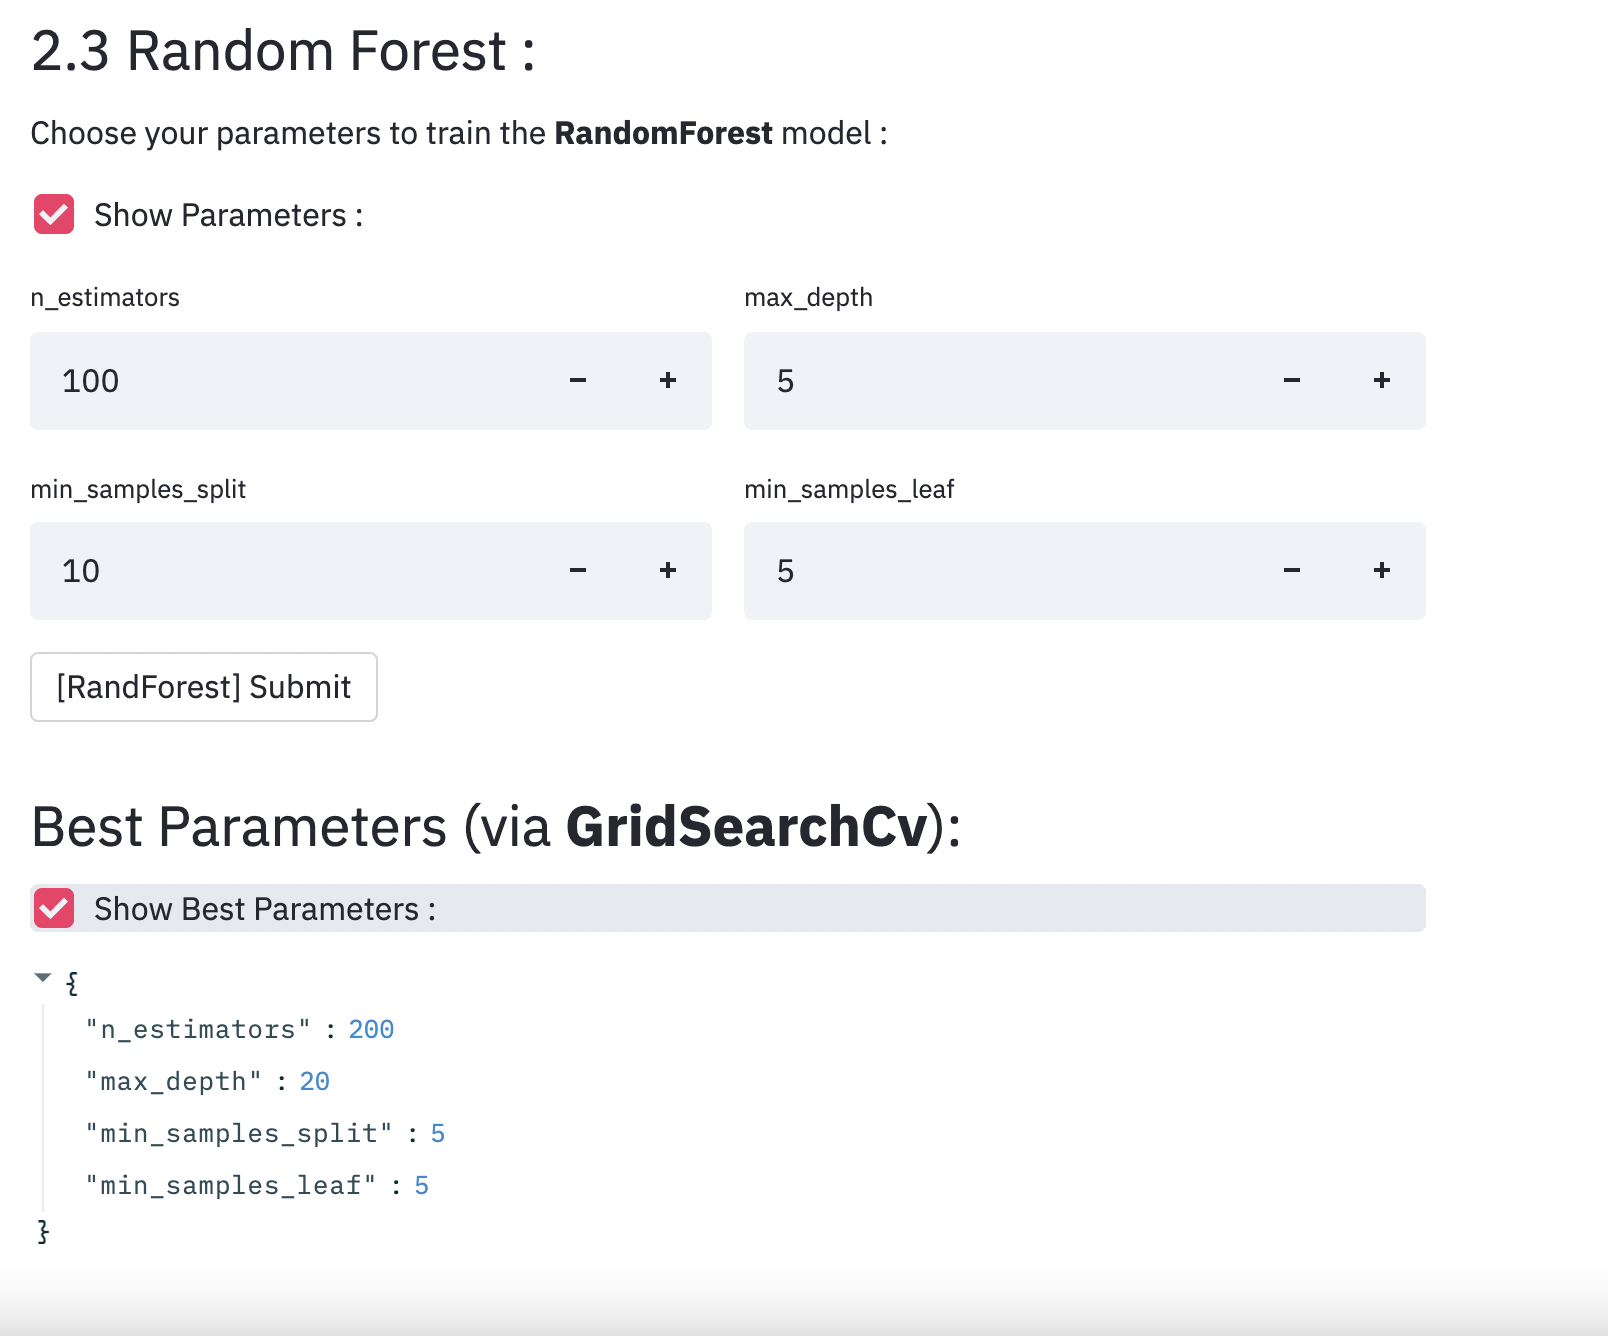
\includegraphics[width=8cm]{src/img/app_5.png} }}
    \qquad
    \subfloat[\centering]{{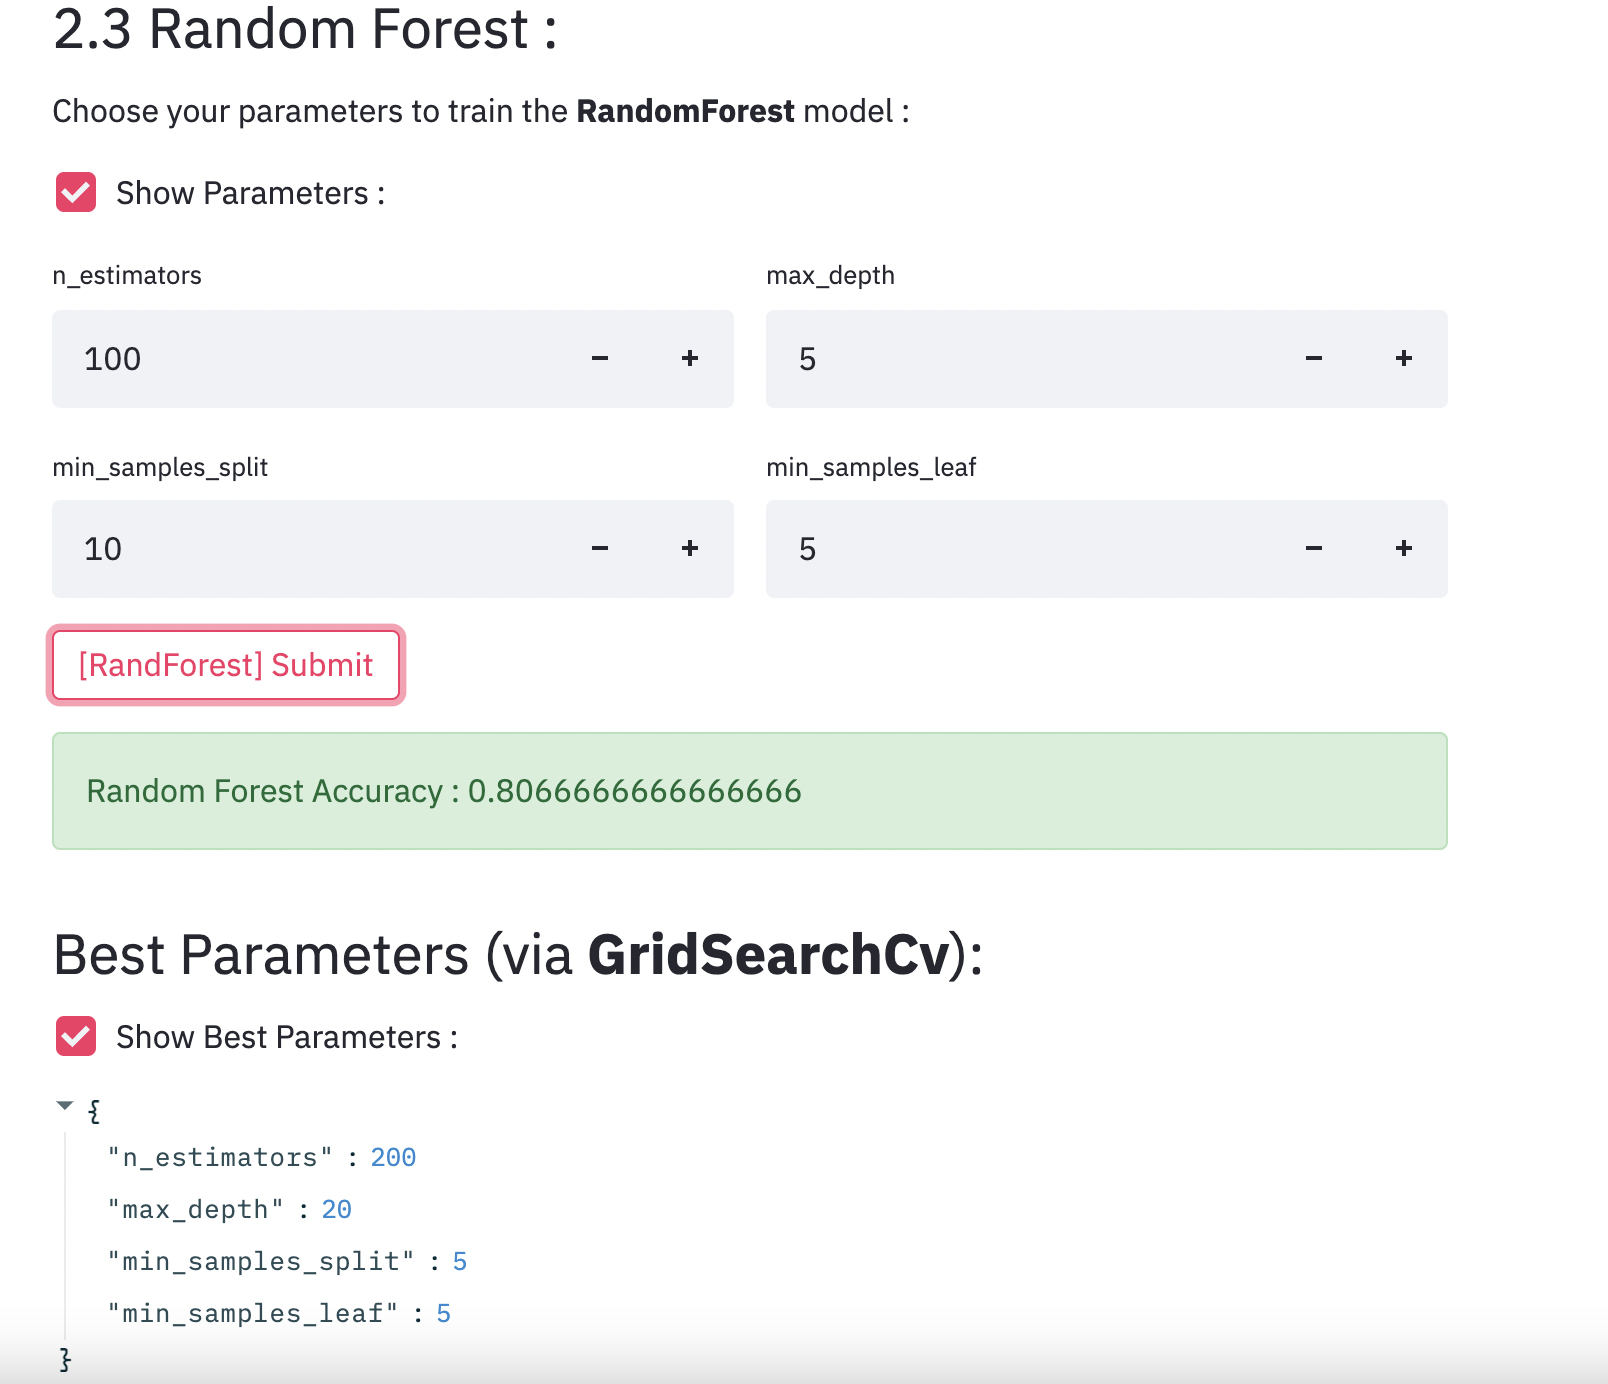
\includegraphics[width=8cm]{src/img/app_6.png} }}
    \caption{Some Screenshot from our website}
    \label{fig:example}
\end{figure}






\newpage
\section*{Conclusions : }
\qquad Online reviews have become a platform for building trust and influencing consumer buying patterns. With such dependency there is a need to handle such large volume of reviews and present credible reviews before the consumer. Our research is aiming to achieve this by conducting sentiment analysis of Amazon products reviews and classifying the reviews into positive and negative,neutral sentiment.Sentiment analysis is one of the most commonly performed NLP tasks as it helps determine overall public opinion about a certain topic.
\\
We performed an analysis of reviews of amazon products using some Machine Learning Models  like SVM (support vector machine),logistic regression ,Knn classifier and Random Forest and we achieved an accuracy of 88\% with the SVM  classifier which was the best accuracy comparing with the accuracy of the Knn Classifier(77\%),logistic regression (85\%) and our last model Random forest(84\%).







\end{document}
